%% LyX 2.4.4 created this file.  For more info, see https://www.lyx.org/.
%% Do not edit unless you really know what you are doing.
\documentclass[12pt,american]{article}
\usepackage[T1]{fontenc}
\usepackage[utf8]{inputenc}
\usepackage{lmodern}
\usepackage{babel}
\usepackage{mathtools}
\usepackage{amsmath}
\usepackage{amsthm}
\usepackage{amssymb}
\usepackage{geometry}
\geometry{verbose,tmargin=2.5cm,bmargin=2.5cm,lmargin=2.5cm,rmargin=2.5cm}
\usepackage{setspace}
\usepackage{microtype}
\usepackage{xcolor}
\usepackage{graphicx}
\usepackage{booktabs}
\usepackage{tabularx,array}
\usepackage{enumitem}
\setlength{\emergencystretch}{3em}
\onehalfspacing
\usepackage[hidelinks,pagebackref]{hyperref}
\allowdisplaybreaks
\numberwithin{equation}{section}

\newtheorem{theorem}{Theorem}[section]
\newtheorem{proposition}[theorem]{Proposition}
\newtheorem{lemma}[theorem]{Lemma}
\newtheorem{corollary}[theorem]{Corollary}
\theoremstyle{definition}
\newtheorem{definition}[theorem]{Definition}
\theoremstyle{remark}
\newtheorem{remark}[theorem]{Remark}

% Reviewer-facing revisions are blue.
\newenvironment{revision}{\begingroup\color{blue}}{\endgroup}

\title{Approximation by mixtures of multivariate Erlang distributions}
\author{Hien Duy Nguyen\\[0.4em]
\small School of Computing, Engineering and Mathematical Sciences, La Trobe University,\\
\small Bundoora, VIC 3086, Australia\\[0.2em]
\small Institute of Mathematics for Industry, Kyushu University,\\
\small Fukuoka 819-0395, Japan}
\date{}

\begin{document}
\maketitle

\begin{abstract}
\begin{revision}
We study finite multivariate Erlang mixtures with a common rate as models for
positive data and actuarial valuation.  A constructive approximation scheme
gives denseness in Lebesgue norms, uniform approximation on compact sets, and
quantitative bounds in terms of the common scale and number of components.
Its mixture weights are probabilities of grid cells.  Estimating these
probabilities through the Bayesian bootstrap produces a finite mixture
posterior whose mean has the deterministic approximation error as its exact
smoothing bias.  Under H\"older regularity and an inverse-moment condition, we
obtain local density-risk bounds at the usual nonparametric rate.  For bounded
actuarial payoffs that are constant outside a compact loss region, we obtain
explicit posterior means and covariances and parametric-order squared-error
bounds after undersmoothing.  Common-rate Erlang convolutions give closed-form
component values for aggregate exceedance probabilities and capped losses.
\end{revision}
\end{abstract}
\par\smallskip\noindent\textbf{Keywords:} multivariate Erlang mixtures; Erlang distributions;
Sz\'asz--Mirakjan--Kantorovich operator; Bayesian bootstrap; density estimation;
actuarial valuation; minimax rate; approximation rates.

\section{Introduction}
\label{sec:introduction}


\begin{revision}
\nopagebreak[4]
Modelling a joint distribution on the positive orthant is a recurring task in
actuarial science, risk theory, reliability, and applied statistics.  Examples
include dependent claim severities, indemnity and allocated loss-adjustment
expenses, aggregate-loss calculations, deductibles and policy limits, and
survival or life-contingency quantities
\cite{Boland2007,KaasGoovaertsDhaeneDenuit2008,KlugmanPanjerWillmot2012,Promislow2015}.
Multivariate Erlang mixtures combine positive-support modelling with
tractable survival,
convolution, and stop-loss calculations.  In particular,
\cite{LeeLin2012} introduced a multivariate common-rate Erlang-mixture class and
established weak denseness, while subsequent work developed likelihood fitting,
censoring methods, penalised estimation, and structural insurance calculations
\cite{GuiHuangLin2021,VerbelenAntonioClaeskens2016,WillmotLin2011,WillmotWoo2015,YinEtAl2019}.
Bayesian positive-support mixture modelling includes gamma-mixture priors for
density estimation and structured common-scale Erlang basis priors for
Poisson-process intensities
\cite{BochkinaRousseau2017,KimKottas2022,WiperInsuaRuggeri2001}.
Here we instead apply an Erlang smoothing map to the Bayesian-bootstrap
posterior of the sampling distribution, so that the approximation bounds
control the smoothing bias of a fitted mixture.

Our work addresses two linked questions.  How accurately can a multivariate
density on $\mathbb{R}_{+}^{d}$ be approximated by a finite common-rate Erlang
mixture, and what do these bounds imply when the mixture is estimated from
observations?  The one-dimensional Sz\'asz--Mirakjan--Kantorovich operator \cite[Section~2]{AltomareCappellettiLeonessa2013},
its coordinatewise product, and a truncation argument give $L^{p}$ denseness,
compact-uniform and weighted approximation, and rates indexed by the common
scale and number of components.  The mixture coefficients are probabilities
of grid cells, which provides the connection to estimation.

For continuous payoff functions, weak convergence and uniform integrability of
the payoffs ensure convergence of expected values.  Density-level approximation
also controls classes of events and bounded contracts simultaneously.  For
example, the total variation distance between distributions with densities $g$
and $f$ is $\|g-f\|_{1}/2$.  Compact-uniform approximation controls any bounded
valuation function whose nonconstant part is supported in the compact region.
This includes aggregate exceedance probabilities, limited expected losses, and
capped stop-loss layers.

The statistical construction replaces the unknown cell probabilities by their
Bayesian-bootstrap counterparts \cite{Rubin1981}.  For $N$ observations, each
posterior draw is a common-rate Erlang mixture with at most $N$ distinct
components.  The posterior mean uses the empirical cell frequencies and
requires neither latent-component sampling nor numerical mixture optimisation.
Its frequentist expectation is exactly the approximation operator applied to
the true density.  The deterministic approximation error is therefore the
bias of this fitted estimator.

For bounded densities that are locally H\"older of order $\alpha\in(0,1]$, the
compact approximation bound gives local squared $L^2$ bias of order
$n^{-\alpha}$, where $n$ is the common Erlang rate.  Under an inverse
half-moment condition, the Erlang-kernel norm bound gives a variance term of
order $n^{d/2}/N$.  Balancing these terms yields the local squared density-risk
order $N^{-2\alpha/(2\alpha+d)}$.  The same order holds for the integrated
posterior loss.  The exponent is minimax when the density class contains a
nontrivial H\"older ball supported in an interior cube \cite{Tsybakov2009}.

For bounded actuarial valuations that are constant outside a compact loss
region, the posterior mean and covariance are explicit Dirichlet-weight
calculations.  The squared-error bound has order $n^{-\alpha}+N^{-1}$, so
$n\asymp N^{1/\alpha}$ is sufficient for the parametric order $N^{-1}$.
Common-rate Erlang convolutions give closed-form component values for
aggregate exceedance probabilities, limited expected losses, capped stop-loss
layers, and lower-orthant probabilities.

Related approximation results include the one-dimensional $L^p$ convergence
and weighted approximation theory for generalized
Sz\'asz--Mirakjan--Kantorovich operators
\cite{AltomareCappellettiLeonessa2013} and the smoothness characterizations of
$L^p$ approximation orders in \cite{Totik1983}.  For Bayesian density
estimation on the positive half-line, \cite{BochkinaRousseau2017} approximate
locally H\"older densities by gamma mixtures and derive adaptive $L^1$
posterior contraction rates that are minimax up to logarithmic factors under
their regularity and tail conditions.  Their gamma-mixture prior differs from
smoothing the Bayesian-bootstrap distribution at a specified resolution.
The latter construction allows the deterministic approximation bounds to be
combined with Dirichlet-weight identities for density and valuation risk.

The remainder of the paper is organised as follows.
Section~\ref{sec:notation} defines the Erlang kernels and tensorized operator.
Sections~\ref{sec:qualitative} and~\ref{sec:scale-rates} state the core
approximation results used later.  Section~\ref{sec:bayesian-estimation}
constructs the Bayesian-bootstrap Erlang posterior and proves its local density
risk.  Section~\ref{sec:actuarial-functionals} develops the actuarial
functionals and their closed-form component valuations.
Section~\ref{sec:numerical-demonstration} illustrates the density-risk
decomposition and joint inference for two bounded actuarial quantities.
Section~\ref{sec:discussion} relates the results to published fitting examples
and discusses further applications.  Appendix~\ref{app:additional-approximation}
contains the additional weighted and component-count results, including the
kernel norm bound used for density risk.  The proofs are collected in
Appendices~\ref{sec:proofs} and~\ref{app:bayesian-proofs}.
\end{revision}
\section{Notation and technical preliminaries}

\label{sec:notation}

Throughout, $\mathbb{N}=\{1,2,\dots\}$, $\mathbb{N}_{0}=\{0,1,2,\dots\}$,
and $\mathbb{R}_{+}=[0,\infty)$. For $x=(x_{1},\dots,x_{d})\in\mathbb{R}_{+}^{d}$,
we write 
\[
\left\lVert x\right\rVert _{1}=\sum_{j=1}^{d}\left\lvert x_{j}\right\rvert ,\qquad\left\lVert x\right\rVert _{2}=\left(\sum_{j=1}^{d}x_{j}^{2}\right)^{1/2}.
\]
If $j\in\{1,\dots,d\}$, then $x=(x_{j},x_{-j})$ denotes the decomposition
into the $j$th coordinate and the remaining $(d-1)$ coordinates.

\begin{definition} For $d\in\mathbb{N}$ and $1\le p<\infty$, define
\[
\mathcal{D}_{p}(\mathbb{R}_{+}^{d})=\left\{ f\in L^{p}(\mathbb{R}_{+}^{d}):f\ge0\ \text{a.e.\ and }\int_{\mathbb{R}_{+}^{d}}f(x)\,\mathrm{d}x=1\right\}.
\]
Thus $\mathcal{D}_{p}(\mathbb{R}_{+}^{d})$ is the class of probability
densities on $\mathbb{R}_{+}^{d}$ that also belong to $L^{p}(\mathbb{R}_{+}^{d})$.
\end{definition}

For $m\in\mathbb{N}$ and $\beta>0$, let 
\begin{equation}
\tau_{m,\beta}(x)=\frac{\beta(\beta x)^{m-1}e^{-\beta x}}{(m-1)!},\qquad x\ge0.\label{eq:erlang-density-beta}
\end{equation}
This is the Erlang density with integer shape parameter $m$ and rate
$\beta$ (equivalently, scale $1/\beta$). When $\beta=n\in\mathbb{N}$,
we write simply 
\begin{equation}
\tau_{m,n}(x)=ne^{-nx}\frac{(nx)^{m-1}}{(m-1)!},\qquad x\ge0.\label{eq:erlang-density-n}
\end{equation}

\begin{definition} A finite multivariate Erlang mixture density with common
rate $\beta$ is a density of the form 
\begin{equation}
g(x)=\sum_{m\in F}a_{m}\prod_{j=1}^{d}\tau_{m_{j},\beta}(x_{j}),\qquad x\in\mathbb{R}_{+}^{d},\label{eq:finite-mixed-erlang}
\end{equation}
where $F\subset\mathbb{N}^{d}$ is finite, $a_{m}\ge0$, and $\sum_{m\in F}a_{m}=1$.
\end{definition}

For later use, fix $M>0$ and write $Q_{M}=[0,M]^{d}$. If $r>0$
and $f$ is bounded on $Q_{M+r}$, define the local modulus of continuity
on $Q_{M+r}$ by 
\begin{equation}
\omega_{Q_{M+r}}(f;r)=\sup\left\{\left\lvert f(y)-f(z)\right\rvert :y,z\in Q_{M+r},\ \left\lVert y-z\right\rVert _{2}\le r\right\}.\label{eq:local-modulus}
\end{equation}

For $\nu\ge0$, define the polynomial weight 
\begin{equation}
w_{\nu}(x)=(1+\left\lVert x\right\rVert _{1})^{\nu},\qquad x\in\mathbb{R}_{+}^{d},\label{eq:poly-weight}
\end{equation}
and the corresponding weighted spaces 
\begin{equation}
L_{\infty,\nu}(\mathbb{R}_{+}^{d})=\left\{ f:\mathbb{R}_{+}^{d}\to\mathbb{R}\ \text{measurable}:\left\lVert f\right\rVert _{\infty,\nu}<\infty\right\},\qquad\left\lVert f\right\rVert _{\infty,\nu}=\sup_{x\in\mathbb{R}_{+}^{d}}\frac{\left\lvert f(x)\right\rvert }{w_{\nu}(x)},\label{eq:weighted-sup-space}
\end{equation}
and, for $1\le p<\infty$ and $\eta\ge0$, 
\begin{equation}
L_{p,\eta}(\mathbb{R}_{+}^{d})=L^{p}(\mathbb{R}_{+}^{d},w_{\eta}(x)^{-1}\,\mathrm{d}x),\qquad\left\lVert f\right\rVert _{p,\eta}=\left(\int_{\mathbb{R}_{+}^{d}}\frac{\left\lvert f(x)\right\rvert ^{p}}{w_{\eta}(x)}\,\mathrm{d}x\right)^{1/p}.\label{eq:weighted-lp-space}
\end{equation}
We also write $C_{0}(\mathbb{R}_{+}^{d})$ for the space of bounded
continuous functions on $\mathbb{R}_{+}^{d}$ that vanish at infinity,
that is, satisfy $f(x)\to0$ as $\left\lVert x\right\rVert _{1}\to\infty$.

The global weighted rate statements use an operator-adapted Hölder
seminorm. For $\nu\ge0$ and $0<\alpha\le1$, define 
\begin{equation}
[f]_{\nu,\alpha,*}=\sup\left\{ \frac{\left\lvert f(y)-f(x)\right\rvert }{w_{\nu}(x)\left(\frac{\left\lVert y-x\right\rVert _{2}}{\sqrt{1+\left\lVert x\right\rVert _{1}}}\right)^{\alpha}}:x,y\in\mathbb{R}_{+}^{d},\ y\neq x\right\} .\label{eq:weighted-holder-seminorm}
\end{equation}
We also define the intrinsic weighted modulus of continuity 
\begin{equation}
\Omega_{\nu,*}(f;\delta)=\sup\left\{ \frac{\left\lvert f(y)-f(x)\right\rvert }{w_{\nu}(x)}:x,y\in\mathbb{R}_{+}^{d},\ \left\lVert y-x\right\rVert _{2}\le\delta\sqrt{1+\left\lVert x\right\rVert _{1}}\right\} ,\qquad\delta>0.\label{eq:intrinsic-modulus-def}
\end{equation}
The weight $w_{\nu}$ permits polynomial growth of order $\nu$ at
infinity. \textcolor{blue}{The scale $\delta\sqrt{1+\left\lVert x\right\rVert _{1}}$
in $\Omega_{\nu,*}$ reflects the displacement bound in
Proposition~\ref{prop:prob-representation} and Lemma~\ref{lem:displacement-moments}.
The second moment of $Y_{n,x}-x$ is bounded above by a constant times
$(1+\left\lVert x\right\rVert _{1})/n$, so
$\sqrt{(1+\left\lVert x\right\rVert _{1})/n}$ bounds the root mean squared displacement up to a constant
depending only on $d$.} \textcolor{blue}{Weighted norms and moduli of smoothness are used in approximation
on unbounded intervals and for positive operators on the half-line
\cite{AltomareCappellettiLeonessa2013,DitzianTotik1987}.}

The one-dimensional Szász--Mirakjan--Kantorovich operator is given
by 
\begin{equation}
(K_{n}g)(x)=n\sum_{k=0}^{\infty}e^{-nx}\frac{(nx)^{k}}{k!}\int_{k/n}^{(k+1)/n}g(t)\,\mathrm{d}t,\qquad x\ge0.\label{eq:Kn-def-main}
\end{equation}
The one-dimensional input is the following result.

\begin{theorem}[One-dimensional $L^p$ convergence; Theorem 3.5 of \cite{AltomareCappellettiLeonessa2013}]\label{thm:1d-input}
Let $1\le p<\infty$. For every $n\in\mathbb{N}$, the operator $K_{n}$
maps $L^{p}(\mathbb{R}_{+})$ into itself, is a positive linear contraction,
and satisfies $\left\lVert K_{n}g\right\rVert _{L^{p}(\mathbb{R}_{+})}\le\left\lVert g\right\rVert _{L^{p}(\mathbb{R}_{+})}$
for every $g\in L^{p}(\mathbb{R}_{+})$. Moreover, $\left\lVert K_{n}g-g\right\rVert _{L^{p}(\mathbb{R}_{+})}\to0$
as $n\to\infty$ for every $g\in L^{p}(\mathbb{R}_{+})$. \end{theorem}

\begin{proposition}[One-dimensional Erlang mixture representation]\label{prop:1d-representation}
Let $1\le p<\infty$ and $f\in\mathcal{D}_{p}(\mathbb{R}_{+})$. For
each $n\in\mathbb{N}$, define 
\begin{equation}
a_{m,n}=\int_{(m-1)/n}^{m/n}f(t)\,\mathrm{d}t,\qquad m\in\mathbb{N}.\label{eq:1d-cell-mass}
\end{equation}
Then $a_{m,n}\ge0$, $\sum_{m=1}^{\infty}a_{m,n}=1$, and 
\begin{equation}
(K_{n}f)(x)=\sum_{m=1}^{\infty}a_{m,n}\,\tau_{m,n}(x),\qquad x\ge0.\label{eq:1d-mixed-erlang-representation}
\end{equation}
Hence $K_{n}f$ is a countable Erlang mixture density with common
scale $1/n$. \end{proposition}

For $d\in\mathbb{N}$ and $j\in\{1,\dots,d\}$, define the coordinatewise
lifted operator 
\begin{equation}
(K_{n,j}f)(x)=n\sum_{k=0}^{\infty}e^{-nx_{j}}\frac{(nx_{j})^{k}}{k!}\int_{k/n}^{(k+1)/n}f(x_{1},\dots,x_{j-1},t,x_{j+1},\dots,x_{d})\,\mathrm{d}t.\label{eq:Knj-def-main}
\end{equation}
We then define the tensorized operator 
\begin{equation}
\mathcal{K}_{n}^{(d)}=K_{n,1}\circ K_{n,2}\circ\cdots\circ K_{n,d}.\label{eq:Kd-def-main}
\end{equation}

\begin{revision}
Here and below, tensorized means that the same one-dimensional smoothing
operation is applied successively in each coordinate.  This coordinatewise
product construction is also used for bivariate Sz\'asz--Mirakjan--Kantorovich
operators in \cite[Section~3, Lemma~3.1]{BarbosuEtAl2010}.  Equivalently,
the resulting multivariate kernels are products of one-dimensional Erlang
densities.  For example, when $d=2$, Proposition~\ref{prop:explicit-mixed-erlang}
gives
\[
 (\mathcal K_n^{(2)}f)(x_1,x_2)
 =\sum_{m_1,m_2\geq1}a_{(m_1,m_2),n}
   \tau_{m_1,n}(x_1)\tau_{m_2,n}(x_2).
\]
The product form of each component does not impose independence on the target
law because dependence is represented by the joint cell-weight array
$\{a_{(m_1,m_2),n}\}$, which need not factorize into marginal weights.
\end{revision}
The operator admits a useful probabilistic representation.

\begin{proposition}[A probabilistic representation]\label{prop:prob-representation}
Fix $d\in\mathbb{N}$, $n\in\mathbb{N}$, and $x=(x_{1},\dots,x_{d})\in\mathbb{R}_{+}^{d}$.
Let $N_{1},\dots,N_{d}$ be independent Poisson random variables with
$N_{j}\sim\mathrm{Poisson}(nx_{j})$, and let $U_{1},\dots,U_{d}$
be independent ${\rm Unif}[0,1]$ random variables, independent of
the $N_{j}$. Define $Y_{n,x,j}=(N_{j}+U_{j})/n$ for $j=1,\dots,d$
and write $Y_{n,x}=(Y_{n,x,1},\dots,Y_{n,x,d})$. Then, for every
measurable and locally integrable $f:\mathbb{R}_{+}^{d}\to\mathbb{R}$
such that $\mathbb{E}[|f(Y_{n,x})|]<\infty$,
\begin{equation}
(\mathcal{K}_{n}^{(d)}f)(x)=\mathbb{E}[f(Y_{n,x})].\label{eq:prob-representation-main}
\end{equation}
\end{proposition}

\begin{lemma}[Moments of the displacement]\label{lem:displacement-moments}
Let $\Delta_{n,x}=Y_{n,x}-x$. Then, for every $x\in\mathbb{R}_{+}^{d}$,
\begin{equation}
\mathbb{E}\left[\left\lVert \Delta_{n,x}\right\rVert _{2}^{2}\right]=\frac{\left\lVert x\right\rVert _{1}}{n}+\frac{d}{3n^{2}}.\label{eq:second-moment-displacement-main}
\end{equation}
Consequently, for every $0<r\le2$, 
\begin{equation}
\mathbb{E}\left[\left\lVert \Delta_{n,x}\right\rVert _{2}^{r}\right]\le C_{r,d}\left(\frac{1+\left\lVert x\right\rVert _{1}}{n}\right)^{r/2},\label{eq:r-moment-displacement-main}
\end{equation}
where one may take $C_{r,d}=(1+d/3)^{r/2}$. Finally, for every $\eta>0$,
\begin{equation}
\mathbb{P}\left(\left\lVert \Delta_{n,x}\right\rVert _{2}>\eta\right)\le\frac{1}{\eta^{2}}\left(\frac{\left\lVert x\right\rVert _{1}}{n}+\frac{d}{3n^{2}}\right).\label{eq:tail-displacement-main}
\end{equation}
\end{lemma}

\begin{lemma}[Weighted moments of $Y_{n,x}$]\label{lem:weighted-moments}
Let $\nu\ge0$. Then there exists a constant $A_{\nu,d}>0$ such that
\begin{equation}
\mathbb{E}[w_{\nu}(Y_{n,x})]\le A_{\nu,d}\,w_{\nu}(x)\qquad(x\in\mathbb{R}_{+}^{d},\ n\in\mathbb{N}).\label{eq:weighted-moment-bound-main}
\end{equation}
Consequently, 
\begin{equation}
\left\lVert \mathcal{K}_{n}^{(d)}f\right\rVert _{\infty,\nu}\le A_{\nu,d}\,\left\lVert f\right\rVert _{\infty,\nu}\qquad(f\in L_{\infty,\nu}(\mathbb{R}_{+}^{d}),\ n\in\mathbb{N}).\label{eq:weighted-operator-bound-main}
\end{equation}
\end{lemma}

\begin{remark}
Observe that (\ref{eq:prob-representation-main}) holds for every bounded measurable $f$
and, by Lemma~\ref{lem:weighted-moments}, for every $f\in L_{\infty,\nu}(\mathbb{R}_{+}^{d})$,
$\nu\ge0$. 
\end{remark}

\section{Qualitative approximation theorems}

\label{sec:qualitative}

We begin with the basic $L^{p}$ approximation theorem for the tensorized
operator.

\begin{theorem}[Tensorized $L^p$ convergence]\label{thm:tensor-convergence}
Let $d\in\mathbb{N}$ and $1\le p<\infty$. Then, for every $f\in L^{p}(\mathbb{R}_{+}^{d})$,
\[
\left\lVert \mathcal{K}_{n}^{(d)}f-f\right\rVert _{L^{p}(\mathbb{R}_{+}^{d})}\longrightarrow0\qquad(n\to\infty).
\]
Moreover, for every $n\in\mathbb{N}$, the operator $\mathcal{K}_{n}^{(d)}$
is a positive linear contraction on $L^{p}(\mathbb{R}_{+}^{d})$.
\end{theorem}

\textcolor{blue}{For a probability density $f$, the next proposition gives a countable
Erlang mixture representation of $\mathcal{K}_{n}^{(d)}f$.}

\begin{proposition}[Multivariate Erlang mixture formula]\label{prop:explicit-mixed-erlang}
Let $d\in\mathbb{N}$, let $1\le p<\infty$, and let $f\in\mathcal{D}_{p}(\mathbb{R}_{+}^{d})$.
For $m=(m_{1},\dots,m_{d})\in\mathbb{N}^{d}$ and $n\in\mathbb{N}$,
define 
\begin{equation}
\textcolor{blue}{\mathcal C_{m,n}}=\prod_{j=1}^{d}\left[\frac{m_{j}-1}{n},\frac{m_{j}}{n}\right)\label{eq:cells-main}
\end{equation}
and the corresponding cell mass 
\begin{equation}
a_{m,n}=\int_{\textcolor{blue}{\mathcal C_{m,n}}}f(t)\,\mathrm{d}t.\label{eq:cell-masses-main}
\end{equation}
Then $a_{m,n}\ge0$, $\sum_{m\in\mathbb{N}^{d}}a_{m,n}=1$, and 
\begin{equation}
(\mathcal{K}_{n}^{(d)}f)(x)=\sum_{m\in\mathbb{N}^{d}}a_{m,n}\prod_{j=1}^{d}\tau_{m_{j},n}(x_{j}),\qquad x\in\mathbb{R}_{+}^{d}.\label{eq:multivariate-representation-main}
\end{equation}
Consequently, $\mathcal{K}_{n}^{(d)}f$ is a countable multivariate
Erlang mixture density with common rate $\beta_{n}=n$ (equivalently, common
scale $1/n$). \end{proposition}

\begin{corollary}[Countable Erlang mixture approximation]\label{cor:countable}
Let $d\in\mathbb{N}$ and $1\le p<\infty$. For every $f\in\mathcal{D}_{p}(\mathbb{R}_{+}^{d})$,
the sequence $\mathcal{K}_{n}^{(d)}f$ consists of countable multivariate
Erlang mixture densities with common scale parameter $1/n$ and satisfies
\[
\left\lVert \mathcal{K}_{n}^{(d)}f-f\right\rVert _{L^{p}(\mathbb{R}_{+}^{d})}\to0.
\]
\end{corollary}

\begin{corollary}[Finite mixture via compact support]\label{cor:compact-finite}
Let $1\le p<\infty$ and let $f\in\mathcal{D}_{p}(\mathbb{R}_{+}^{d})$
vanish a.e. on $\mathbb{R}_{+}^{d}\setminus Q_{M}$ for some $M>0$. Then,
for every $n\in\mathbb{N}$, the Erlang mixture approximation $\mathcal{K}_{n}^{(d)}f$
is already a finite multivariate Erlang mixture density. More precisely,
only indices $m=(m_{1},\dots,m_{d})$ with $1\le m_{j}\le\lfloor nM\rfloor+1$
can appear in \eqref{eq:multivariate-representation-main}. \end{corollary}

The main qualitative density theorem is the following finite-mixture version.

\begin{theorem}[Finite multivariate Erlang mixture approximation]\label{thm:finite-approx}
Let $d\in\mathbb{N}$ and $1\le p<\infty$. Then the class of finite
multivariate Erlang mixture densities with common scale parameter
is dense in $\mathcal{D}_{p}(\mathbb{R}_{+}^{d})$ with respect to
the $L^{p}(\mathbb{R}_{+}^{d})$ norm. More explicitly, if $f\in\mathcal{D}_{p}(\mathbb{R}_{+}^{d})$,
then there exists a sequence $(g_{n})_{n\ge1}$ of finite multivariate
Erlang mixture densities such that 
\[
\left\lVert g_{n}-f\right\rVert _{L^{p}(\mathbb{R}_{+}^{d})}\longrightarrow0.
\]
Moreover, the common scale parameter of $g_{n}$ may be chosen to
be $1/n$. \end{theorem}

\begin{remark}\label{rem:gamma} Let $d\in\mathbb{N}$ and $1\le p<\infty$.
Any class of densities on $\mathbb{R}_{+}^{d}$ that contains all
finite mixtures of product-Erlang densities is $L^{p}$-dense in $\mathcal{D}_{p}(\mathbb{R}_{+}^{d})$.
In particular, the class of finite mixtures of products of gamma densities
is $L^{p}$-dense in $\mathcal{D}_{p}(\mathbb{R}_{+}^{d})$, because
every Erlang density is a gamma density with integer shape parameter.
\end{remark}

\section{Convergence rates in scale}

\label{sec:scale-rates}

The compact-set sup-norm estimate underlying the local uniform theory is as follows.

\begin{theorem}[Compact-set $L^\infty$ bound]\label{thm:compact-modulus}
Let $M>0$ and let $f:\mathbb{R}_{+}^{d}\to\mathbb{R}$ be bounded
and continuous. Then, for every $r>0$ and every $n\in\mathbb{N}$,
\begin{equation}
\left\lVert \mathcal{K}_{n}^{(d)}f-f\right\rVert _{L^{\infty}(Q_{M})}\le\omega_{Q_{M+r}}(f;r)+\frac{2\left\lVert f\right\rVert _{L^{\infty}(\mathbb{R}_{+}^{d})}}{r^{2}}\left(\frac{dM}{n}+\frac{d}{3n^{2}}\right).\label{eq:compact-modulus-estimate-main}
\end{equation}
\end{theorem}

\begin{corollary}[Local uniform convergence on compact sets]\label{cor:compact-uniform}
If $f$ is bounded and continuous on $\mathbb{R}_{+}^{d}$, then for
every $M>0$, 
\[
\left\lVert \mathcal{K}_{n}^{(d)}f-f\right\rVert _{L^{\infty}(Q_{M})}\longrightarrow0\qquad(n\to\infty).
\]
\end{corollary}

\begin{theorem}[Compact-set H\"older rate]\label{thm:compact-holder}
Let $M>0$, let $0<\alpha\le1$, and let $f:\mathbb{R}_{+}^{d}\to\mathbb{R}$
be bounded and measurable. Assume that there is a constant $H>0$ such that 
\begin{equation}
\left\lvert f(y)-f(z)\right\rvert \le H\left\lVert y-z\right\rVert _{2}^{\alpha}\qquad(y,z\in Q_{M+1}).\label{eq:local-holder-compact-main}
\end{equation}
Then, for every $n\in\mathbb{N}$, 
\begin{equation}
\left\lVert \mathcal{K}_{n}^{(d)}f-f\right\rVert _{L^{\infty}(Q_{M})}\le HC_{\alpha,d}\left(\frac{1+dM}{n}\right)^{\alpha/2}+2\left\lVert f\right\rVert _{L^{\infty}(\mathbb{R}_{+}^{d})}\left(\frac{dM}{n}+\frac{d}{3n^{2}}\right),\label{eq:compact-holder-rate-main}
\end{equation}
where one may take $C_{\alpha,d}=(1+d/3)^{\alpha/2}$. In particular,
\[
\left\lVert \mathcal{K}_{n}^{(d)}f-f\right\rVert _{L^{\infty}(Q_{M})}=O(n^{-\alpha/2}).
\]
\end{theorem}


\section{Bayesian estimation from the approximation theory}
\label{sec:bayesian-estimation}

\begin{revision}
Throughout this section, $X_{1},\ldots,X_{N}$ are independent observations
from a probability density $f$ on $\mathbb{R}_{+}^{d}$.  For
$x\in\mathbb{R}_{+}^{d}$, define
\begin{equation}
 m_{n}(x)=\bigl(1+\lfloor nx_{1}\rfloor,\ldots,
                   1+\lfloor nx_{d}\rfloor\bigr)
 \quad\text{and}\quad
 \varphi_{n,x}(y)=\prod_{j=1}^{d}
 \tau_{m_{n,j}(x),n}(y_{j}).
 \label{eq:data-kernel}
\end{equation}
The map $x\mapsto\varphi_{n,x}$ is constant on each cell $\mathcal C_{m,n}$.

\subsection{Smoothing probability measures and transferring oracle error}

For any probability measure $P$ on $\mathbb{R}_{+}^{d}$, define its
Erlang-smoothed density by
\begin{equation}
 (\mathcal{E}_{n}P)(y)
 =\int_{\mathbb{R}_{+}^{d}}\varphi_{n,x}(y)\,P(\mathrm{d}x)
 =\sum_{m\in\mathbb{N}^{d}}P(\mathcal C_{m,n})\varphi_{m,n}(y),
 \label{eq:measure-smoothing-map}
\end{equation}
where $\varphi_{m,n}(y)=\prod_{j=1}^{d}\tau_{m_{j},n}(y_{j})$.
The second equality follows by partitioning the $x$-integral over the cells.
For a bounded measurable valuation function $\psi$ and a density $g$, write
\begin{equation}
 \Theta_{\psi}(g)=\int_{\mathbb{R}_{+}^{d}}\psi(y)g(y)\,\mathrm{d}y.
 \label{eq:valuation-functional}
\end{equation}

\begin{proposition}[Measure smoothing and a fixed-grid transfer inequality]
\label{prop:measure-smoothing-transfer}
For every probability measure $P$, $\mathcal{E}_{n}P$ is a countable
common-rate multivariate Erlang-mixture density.  If $P$ has density $f$, then
\begin{equation}
 \mathcal{E}_{n}P=\mathcal{K}_{n}^{(d)}f.
 \label{eq:smoothing-equals-operator}
\end{equation}
If $P$ and $Q$ are probability measures and
$p_{m}=P(\mathcal C_{m,n})$, $q_{m}=Q(\mathcal C_{m,n})$, then
\begin{equation}
 \|\mathcal{E}_{n}Q-\mathcal{E}_{n}P\|_{L^{1}}
 \leq \sum_{m\in\mathbb{N}^{d}}|q_{m}-p_{m}|.
 \label{eq:cell-weight-transfer}
\end{equation}
Consequently, when $P$ has density $f$,
\begin{equation}
 \|\mathcal{E}_{n}Q-f\|_{L^{1}}
 \leq
 \|\mathcal{K}_{n}^{(d)}f-f\|_{L^{1}}
 +\sum_{m\in\mathbb{N}^{d}}|q_{m}-a_{m,n}|.
 \label{eq:oracle-estimation-decomposition}
\end{equation}
For every bounded measurable valuation function $\psi$,
\begin{align}
 |\Theta_{\psi}(\mathcal{E}_{n}Q)-\Theta_{\psi}(f)|
 &\leq
 |\Theta_{\psi}(\mathcal{K}_{n}^{(d)}f)-\Theta_{\psi}(f)|
 +\|\psi\|_{\infty}
   \sum_{m\in\mathbb{N}^{d}}|q_{m}-a_{m,n}|,
 \label{eq:functional-oracle-estimation-decomposition}
\end{align}
\end{proposition}

Proposition~\ref{prop:measure-smoothing-transfer} gives a direct answer for a
fixed-grid statistical fit.  The approximation results control the first term
in \eqref{eq:oracle-estimation-decomposition}, while a statistical analysis of
the estimated cell weights controls the second.  The Bayesian-bootstrap
construction below instead yields an exact local $L^2$ risk decomposition
for a particular fitted distribution.

\subsection{The Bayesian-bootstrap Erlang posterior}

Let
\begin{equation}
 (W_{1},\ldots,W_{N})\mid X_{1:N}
 \sim\operatorname{Dirichlet}(1,\ldots,1)
 \label{eq:bb-weights}
\end{equation}
independently of all other randomness conditional on the data, and define the
Bayesian-bootstrap draw
$P_{N}^{W}=\sum_{i=1}^{N}W_{i}\delta_{X_{i}}$.
The induced random density and its posterior mean are
\begin{align}
 f_{N,n}^{W}(y)
 &=\mathcal{E}_{n}P_{N}^{W}(y)
 =\sum_{i=1}^{N}W_{i}\varphi_{n,X_{i}}(y),
 \label{eq:bb-erlang-posterior-draw}\\
 \widehat f_{N,n}(y)
 &=\mathbb{E}_{W}[f_{N,n}^{W}(y)\mid X_{1:N}]
 =\frac{1}{N}\sum_{i=1}^{N}\varphi_{n,X_{i}}(y).
 \label{eq:bb-erlang-posterior-mean}
\end{align}
Let $\Pi_{N,n}(\cdot\mid X_{1:N})$ denote the conditional distribution of
$f_{N,n}^{W}$ induced by the Dirichlet weights in
\eqref{eq:bb-weights}.

\begin{proposition}[Finite posterior mixture and oracle mean]
\label{prop:bb-finite-oracle}
Conditional on the data, every $f_{N,n}^{W}$ is a finite multivariate Erlang
mixture density with common rate $n$ and at most $N$ distinct components.  If
$C_{m}=\sum_{i=1}^{N}\mathbf{1}\{X_{i}\in \mathcal C_{m,n}\}$, then the aggregated
posterior weights on the occupied cells have a Dirichlet distribution with
parameters $(C_{m}:C_{m}>0)$.  Moreover,
\begin{equation}
 \mathbb{E}_{f}[\widehat f_{N,n}(y)]
 =\mathcal{K}_{n}^{(d)}f(y),
 \qquad y\in\mathbb{R}_{+}^{d}.
 \label{eq:posterior-mean-oracle-identity}
\end{equation}
Thus the deterministic approximation error
$\mathcal{K}_{n}^{(d)}f-f$ is exactly the frequentist bias of the posterior
mean.
\end{proposition}

This smoothed Bayesian-bootstrap posterior differs from a prior placed
directly on the weights, shapes, and common rate of an exact finite-mixture
likelihood.  Its risk analysis follows from the Erlang smoothing operator
developed in Sections~\ref{sec:notation}--\ref{sec:scale-rates}.

\begin{lemma}[Dirichlet-weight identity in a Hilbert space]
\label{lem:dirichlet-hilbert}
Let $z_{1},\ldots,z_{N}$ belong to a real Hilbert space $\mathbb{H}$, let
$\overline z=N^{-1}\sum_{i=1}^{N}z_{i}$, and let
$W\sim\operatorname{Dirichlet}(1,\ldots,1)$.  Then
\begin{equation}
 \mathbb{E}_{W}\left\|
 \sum_{i=1}^{N}W_{i}z_{i}-\overline z
 \right\|_{\mathbb{H}}^{2}
 =\frac{1}{N+1}
 \left\{
 \frac{1}{N}\sum_{i=1}^{N}\|z_{i}\|_{\mathbb{H}}^{2}
 -\|\overline z\|_{\mathbb{H}}^{2}
 \right\}.
 \label{eq:dirichlet-hilbert-identity}
\end{equation}
If $Z_{1},\ldots,Z_{N}$ are independent copies of a square-integrable random
element $Z$ with mean $\mu$, the Dirichlet vector $W$ is independent of
$Z_{1:N}$, and $z_{i}=Z_{i}$, then, for every $h\in\mathbb{H}$,
\begin{align}
 \mathbb{E}\|\overline Z-h\|_{\mathbb{H}}^{2}
 &=\|\mu-h\|_{\mathbb{H}}^{2}
   +\frac{1}{N}\mathbb{E}\|Z-\mu\|_{\mathbb{H}}^{2},
 \label{eq:sample-mean-hilbert-risk}\\
 \mathbb{E}\mathbb{E}_{W}
 \left[\left\|\sum_{i=1}^{N}W_{i}Z_{i}-h\right\|_{\mathbb{H}}^{2}
 \middle|Z_{1:N}\right]
 &=\|\mu-h\|_{\mathbb{H}}^{2}
   +\frac{2}{N+1}\mathbb{E}\|Z-\mu\|_{\mathbb{H}}^{2}.
 \label{eq:integrated-bb-hilbert-risk}
\end{align}
\end{lemma}

\subsection{Local density risk and minimax order}

For $M>0$, define the compact approximation bound
\begin{equation}
 \Delta_{n,M}(f;H,\alpha)
 =HC_{\alpha,d}\left(\frac{1+dM}{n}\right)^{\alpha/2}
 +2\|f\|_{\infty}
 \left(\frac{dM}{n}+\frac{d}{3n^{2}}\right),
 \label{eq:delta-compact-bias}
\end{equation}
where $H$ is a H\"older constant satisfying
\eqref{eq:local-holder-compact-main}.  Theorem~\ref{thm:compact-holder}
states that
$\|\mathcal{K}_{n}^{(d)}f-f\|_{L^{\infty}(Q_{M})}
\leq\Delta_{n,M}(f;H,\alpha)$.
We also use the inverse boundary moment
\begin{equation}
 \mu_{-1/2}(f)
 =\int_{\mathbb{R}_{+}^{d}}
   \prod_{j=1}^{d}x_{j}^{-1/2}f(x)\,\mathrm{d}x.
 \label{eq:inverse-half-moment}
\end{equation}
The assumption $\mu_{-1/2}(f)<\infty$ permits mass near zero but excludes
excessively strong singularities on the coordinate boundaries.  It holds, for
example, for bounded densities supported on compact rectangles and for finite
mixtures of product-gamma densities whose coordinatewise shapes exceed $1/2$.
Lemma~\ref{lem:inverse-half-moment-check} verifies these cases and nonsingular
multivariate lognormal densities.

\begin{theorem}[Exact local posterior risk and an explicit bound]
\label{thm:local-bayesian-risk}
Let $M>0$, $0<\alpha\leq1$, and let
$f\in\mathcal{D}_{2}(\mathbb{R}_{+}^{d})$ be bounded.  Suppose that
\eqref{eq:local-holder-compact-main} holds on $Q_{M+1}$ with constant $H$ and
that $\mu_{-1/2}(f)<\infty$.  Set
\begin{equation}
 V_{n,M}(f)
 =\mathbb{E}_{f}\left\|
   \varphi_{n,X}-\mathcal{K}_{n}^{(d)}f
  \right\|_{L^{2}(Q_{M})}^{2}.
 \label{eq:local-kernel-variance}
\end{equation}
Then
\begin{align}
 \mathbb{E}_{f}\|\widehat f_{N,n}-f\|_{L^{2}(Q_{M})}^{2}
 &=\|\mathcal{K}_{n}^{(d)}f-f\|_{L^{2}(Q_{M})}^{2}
   +\frac{V_{n,M}(f)}{N},
 \label{eq:posterior-mean-local-risk-exact}\\
 \mathbb{E}_{f}\mathbb{E}_{W}
 \left[\|f_{N,n}^{W}-f\|_{L^{2}(Q_{M})}^{2}
 \mid X_{1:N}\right]
 &=\|\mathcal{K}_{n}^{(d)}f-f\|_{L^{2}(Q_{M})}^{2}
   +\frac{2V_{n,M}(f)}{N+1}.
 \label{eq:integrated-posterior-local-risk-exact}
\end{align}
Moreover,
\begin{align}
 \mathbb{E}_{f}\|\widehat f_{N,n}-f\|_{L^{2}(Q_{M})}^{2}
 &\leq
 M^{d}\Delta_{n,M}(f;H,\alpha)^{2}
 +\frac{n^{d/2}\mu_{-1/2}(f)}{N},
 \label{eq:posterior-mean-local-risk-bound}\\
 \mathbb{E}_{f}\mathbb{E}_{W}
 \left[\|f_{N,n}^{W}-f\|_{L^{2}(Q_{M})}^{2}
 \mid X_{1:N}\right]
 &\leq
 M^{d}\Delta_{n,M}(f;H,\alpha)^{2}
 +\frac{2n^{d/2}\mu_{-1/2}(f)}{N+1}.
 \label{eq:integrated-posterior-local-risk-bound}
\end{align}
\end{theorem}

For constants $B,H_{0},\mu_{0}>0$, write
\begin{align}
 \mathcal{F}_{\alpha}(M;B,H_{0},\mu_{0})
 =\bigl\{f\in\mathcal{D}_{2}(\mathbb{R}_{+}^{d}):{}
 &\ \|f\|_{\infty}\leq B,\nonumber\\[-0.2em]
 &\ |f(y)-f(z)|\leq H_{0}\|y-z\|_{2}^{\alpha}
     \text{ for }y,z\in Q_{M+1},\nonumber\\[-0.2em]
 &\ \mu_{-1/2}(f)\leq\mu_{0}\bigr\}.
 \label{eq:local-holder-density-class}
\end{align}

\begin{corollary}[Minimax-order local density estimation]
\label{cor:minimax-local-density}
Let $n_{N}=\lceil N^{2/(2\alpha+d)}\rceil$.  There is a constant $C>0$,
depending only on $d,\alpha,M,B,H_{0}$, and $\mu_{0}$, such that
\begin{align}
 \sup_{f\in\mathcal{F}_{\alpha}(M;B,H_{0},\mu_{0})}
 \mathbb{E}_{f}\|\widehat f_{N,n_{N}}-f\|_{L^{2}(Q_{M})}^{2}
 &\leq C N^{-2\alpha/(2\alpha+d)},
 \label{eq:minimax-posterior-mean-rate}\\
 \sup_{f\in\mathcal{F}_{\alpha}(M;B,H_{0},\mu_{0})}
 \mathbb{E}_{f}\mathbb{E}_{W}
 \left[\|f_{N,n_{N}}^{W}-f\|_{L^{2}(Q_{M})}^{2}
 \mid X_{1:N}\right]
 &\leq C N^{-2\alpha/(2\alpha+d)}.
 \label{eq:minimax-integrated-posterior-rate}
\end{align}
If $L_{N}\to\infty$ and
$\varepsilon_{N}=N^{-\alpha/(2\alpha+d)}$, then the induced posterior
$\Pi_{N,n_{N}}$ satisfies
\begin{equation}
 \sup_{f\in\mathcal{F}_{\alpha}(M;B,H_{0},\mu_{0})}
 \mathbb{E}_{f}\Pi_{N,n_{N}}
 \left(\|g-f\|_{L^{2}(Q_{M})}>L_{N}\varepsilon_{N}
 \mid X_{1:N}\right)\longrightarrow0.
 \label{eq:local-posterior-contraction}
\end{equation}
\end{corollary}

\begin{remark}[Minimax interpretation of the local density rate]
\label{rem:minimax-local-density}
Whenever the constants defining
$\mathcal F_{\alpha}(M;B,H_0,\mu_0)$ permit a nontrivial H\"older ball
supported in an interior cube contained in $(0,M)^{d}$, the standard H\"older
minimax lower bound shows that the exponent in
\eqref{eq:minimax-posterior-mean-rate} cannot be improved uniformly
\cite{Tsybakov2009}.
\end{remark}

\end{revision}

\section{Bayesian inference}
\label{sec:actuarial-functionals}

\begin{revision}
\subsection{Exact posterior calculations}

For a bounded measurable valuation function
$\psi:\mathbb{R}_{+}^{d}\to\mathbb{R}$, recall $\Theta_{\psi}$ from
\eqref{eq:valuation-functional} and define
\begin{equation}
 b_{\psi,n}(x)=\int_{\mathbb{R}_{+}^{d}}
 \psi(y)\varphi_{n,x}(y)\,\mathrm{d}y.
 \label{eq:functional-and-component-value}
\end{equation}
Because $\varphi_{n,x}$ is a probability density,
$|b_{\psi,n}(x)|\leq\|\psi\|_{\infty}$.

\begin{proposition}[Posterior mean and covariance of actuarial valuations]
\label{prop:functional-posterior}
For every bounded measurable $\psi$,
\begin{align}
 \Theta_{\psi}(f_{N,n}^{W})
 &=\sum_{i=1}^{N}W_{i}b_{\psi,n}(X_{i}),
 \label{eq:functional-posterior-draw}\\
 \widehat\Theta_{\psi,N,n}
 =\mathbb{E}_{W}[\Theta_{\psi}(f_{N,n}^{W})\mid X_{1:N}]
 &=\frac{1}{N}\sum_{i=1}^{N}b_{\psi,n}(X_{i}).
 \label{eq:functional-posterior-mean}
\end{align}
For bounded valuation functions $\psi_{1},\ldots,\psi_{J}$,
\begin{align}
 &\operatorname{Cov}_{W}\!
 \left\{\Theta_{\psi_{j}}(f_{N,n}^{W}),
        \Theta_{\psi_{k}}(f_{N,n}^{W})\mid X_{1:N}\right\}
 \nonumber\\
 &\quad=\frac{1}{N+1}
 \left\{
 \frac{1}{N}\sum_{i=1}^{N}
 b_{\psi_{j},n}(X_{i})b_{\psi_{k},n}(X_{i})
 -\widehat\Theta_{\psi_{j},N,n}
  \widehat\Theta_{\psi_{k},N,n}
 \right\}.
 \label{eq:functional-posterior-covariance}
\end{align}
Thus one Dirichlet draw gives a joint posterior draw for any finite collection
of retentions, limits, and portfolio events.
\end{proposition}

\subsection{Risk bounds for actuarial estimators}

The relevant class of valuation functions is broader than the
compactly supported class.  Suppose that there are $M>0$ and a constant $c_{\psi}$ such that
\begin{equation}
 \psi-c_{\psi}=0\quad\text{a.e. on }
 \mathbb{R}_{+}^{d}\setminus Q_{M}.
 \label{eq:compact-nonconstant-valuation}
\end{equation}
Since both $f$ and $\mathcal{K}_{n}^{(d)}f$ integrate to one, the constant part
cancels, giving
\begin{equation}
 \Theta_{\psi}(\mathcal{K}_{n}^{(d)}f)-\Theta_{\psi}(f)
 =\int_{Q_{M}}\{\psi(y)-c_{\psi}\}
   \{(\mathcal{K}_{n}^{(d)}f)(y)-f(y)\}\,\mathrm{d}y.
 \label{eq:constant-tail-cancellation}
\end{equation}

\begin{theorem}[Posterior risk for bounded actuarial valuations]
\label{thm:functional-risk}
Let $M>0$, $0<\alpha\leq1$, and let
$f\in\mathcal{D}_{1}(\mathbb{R}_{+}^{d})$ be bounded.  Assume that
\eqref{eq:local-holder-compact-main} holds on $Q_{M+1}$ with constant $H$,
and let $\psi$ be a bounded valuation function satisfying
\eqref{eq:compact-nonconstant-valuation}.  Put
$A_{\psi,M}=\|\psi-c_{\psi}\|_{L^{1}(Q_{M})}$.  Then
\begin{align}
 \mathbb{E}_{f}
 \left[\{\widehat\Theta_{\psi,N,n}-\Theta_{\psi}(f)\}^{2}\right]
 &=\{\Theta_{\psi}(\mathcal{K}_{n}^{(d)}f)-\Theta_{\psi}(f)\}^{2}
   +\frac{\operatorname{Var}_{f}\{b_{\psi,n}(X)\}}{N},
 \label{eq:functional-mean-risk-exact}\\
 \mathbb{E}_{f}\mathbb{E}_{W}
 \left[\{\Theta_{\psi}(f_{N,n}^{W})-\Theta_{\psi}(f)\}^{2}
 \mid X_{1:N}\right]
 &=\{\Theta_{\psi}(\mathcal{K}_{n}^{(d)}f)-\Theta_{\psi}(f)\}^{2}
   +\frac{2\operatorname{Var}_{f}\{b_{\psi,n}(X)\}}{N+1}.
 \label{eq:functional-integrated-risk-exact}
\end{align}
Moreover,
\begin{align}
 \mathbb{E}_{f}
 \left[\{\widehat\Theta_{\psi,N,n}-\Theta_{\psi}(f)\}^{2}\right]
 &\leq A_{\psi,M}^{2}\Delta_{n,M}(f;H,\alpha)^{2}
       +\frac{\|\psi\|_{\infty}^{2}}{N},
 \label{eq:functional-mean-risk-bound}\\
 \mathbb{E}_{f}\mathbb{E}_{W}
 \left[\{\Theta_{\psi}(f_{N,n}^{W})-\Theta_{\psi}(f)\}^{2}
 \mid X_{1:N}\right]
 &\leq A_{\psi,M}^{2}\Delta_{n,M}(f;H,\alpha)^{2}
       +\frac{2\|\psi\|_{\infty}^{2}}{N+1}.
 \label{eq:functional-integrated-risk-bound}
\end{align}
\end{theorem}

\begin{corollary}[Parametric-rate actuarial estimation]
\label{cor:parametric-functional-rate}
Fix $M>0$, $0<\alpha\leq1$, and a bounded valuation function $\psi$ satisfying
\eqref{eq:compact-nonconstant-valuation}.  For constants $B,H_{0}>0$, uniformly
over densities $f\in\mathcal{D}_{1}(\mathbb{R}_{+}^{d})$ satisfying
$\|f\|_{\infty}\leq B$ and
$|f(y)-f(z)|\leq H_{0}\|y-z\|_{2}^{\alpha}$ for $y,z\in Q_{M+1}$, the
choice $n_{N}=\lceil N^{1/\alpha}\rceil$ gives
\begin{equation}
 \mathbb{E}_{f}
 \left[\{\widehat\Theta_{\psi,N,n_{N}}-\Theta_{\psi}(f)\}^{2}\right]
 =O(N^{-1}),
 \label{eq:parametric-functional-mse}
\end{equation}
and the integrated posterior risk has the same order.
\end{corollary}

\begin{remark}[Posterior contraction and minimax interpretation]
\label{rem:functional-consequences}
For every sequence $L_{N}\to\infty$, Markov's inequality applied to the
integrated posterior-risk bound gives, uniformly over the density class in
Corollary~\ref{cor:parametric-functional-rate},
\[
 \mathbb{E}_{f}\Pi_{N,n_{N}}
 \left(\left|\Theta_{\psi}(g)-\Theta_{\psi}(f)\right|>
 L_{N}N^{-1/2}\mid X_{1:N}\right)\longrightarrow0.
\]
On any class containing a regular one-dimensional submodel on which
$\Theta_{\psi}$ is nonconstant, $N^{-1}$ is also the minimax squared-error
order by the usual parametric lower-bound argument
\cite{vanDerVaart1998}.
\end{remark}

The resolution in Corollary~\ref{cor:minimax-local-density} balances the
local density-bias and variance bounds.  The larger resolution used in
Corollary~\ref{cor:parametric-functional-rate} is an undersmoothing choice
that makes the functional-bias bound $O(N^{-1/2})$ while the variance remains
$O(N^{-1})$.  This choice is sufficient for the stated functional-risk
bound.  No Bernstein--von Mises or frequentist credible-interval coverage claim is made
here.

\subsection{Actuarial quantities and closed-form expressions}

Let $s(y)=y_{1}+\cdots+y_{d}$ and
$k_{n}(x)=\sum_{j=1}^{d}m_{n,j}(x)$.  Under the product-Erlang density
$\varphi_{n,x}$, the coordinates are independent conditionally on the
component and have common rate $n$.  Their sum therefore has an
$\operatorname{Erlang}(k_{n}(x),n)$ distribution.  Write
\begin{align}
 \overline G_{k,n}(u)
 &=e^{-nu}\sum_{r=0}^{k-1}\frac{(nu)^{r}}{r!},
 \qquad G_{k,n}(u)=1-\overline G_{k,n}(u),
 \label{eq:erlang-tail-cdf}\\
 \operatorname{SL}_{k,n}(u)
 &=\frac{k}{n}\overline G_{k+1,n}(u)
   -u\overline G_{k,n}(u).
 \label{eq:erlang-stop-loss}
\end{align}
The second expression is the stop-loss expectation
$\mathbb{E}(Z-u)_{+}$ for $Z\sim\operatorname{Erlang}(k,n)$.

\begin{corollary}[Closed-form posterior inputs]
\label{cor:closed-form-actuarial}
For $x\in\mathbb{R}_{+}^{d}$ and $k=k_{n}(x)$, the component values in
\eqref{eq:functional-and-component-value} are as follows.
\begin{enumerate}[label=(\roman*),leftmargin=2.4em]
\item For $u\geq0$, the aggregate exceedance valuation
$\psi_{u}^{\mathrm{exc}}(y)=\mathbf{1}\{s(y)>u\}$,
\begin{equation}
 b_{\psi_{u}^{\mathrm{exc}},n}(x)=\overline G_{k,n}(u).
 \label{eq:component-exceedance}
\end{equation}
Here $c_{\psi}=1$.  If $u>0$, one may take $M=u$, and
$A_{\psi,u}=u^{d}/d!$ because the nonconstant part is the negative indicator
of the simplex $\{s\leq u\}$.  If $u=0$, the valuation is equal to one
almost everywhere and the same formula gives $A_{\psi,0}=0$.

\item For $u\geq0$, the aggregate limited-loss payoff
$\psi_{u}^{\mathrm{LEV}}(y)=\min\{s(y),u\}$ has component value
\begin{equation}
 b_{\psi_{u}^{\mathrm{LEV}},n}(x)
 =\frac{k}{n}G_{k+1,n}(u)+u\overline G_{k,n}(u)
 =\frac{k}{n}-\operatorname{SL}_{k,n}(u).
 \label{eq:component-lev}
\end{equation}
Here $c_{\psi}=u$.  If $u>0$, one may take $M=u$ and
$A_{\psi,u}=u^{d+1}/(d+1)!$.  If $u=0$, the valuation is identically zero and
the same formula gives $A_{\psi,0}=0$.

\item For the capped aggregate stop-loss or layer valuation with attachment
$u\geq0$ and limit $v>0$,
\[
 \psi_{u,v}^{\mathrm{layer}}(y)
 =\min\{(s(y)-u)_{+},v\},
\]
\begin{equation}
 b_{\psi_{u,v}^{\mathrm{layer}},n}(x)
 =\operatorname{SL}_{k,n}(u)-\operatorname{SL}_{k,n}(u+v).
 \label{eq:component-layer}
\end{equation}
Here $c_{\psi}=v$, one may take $M=u+v$, and
\begin{equation}
 A_{\psi,u,v}=A_{\psi,M}
 =\frac{(u+v)^{d+1}-u^{d+1}}{(d+1)!}.
 \label{eq:layer-bias-constant}
\end{equation}

\item For $t=(t_1,\ldots,t_d)\in\mathbb R_+^d$, the lower-orthant indicator
$\psi_{t}^{\mathrm{orth}}(y)=
\mathbf{1}\{y_{1}\leq t_{1},\ldots,y_{d}\leq t_{d}\}$ has component value
\begin{equation}
 b_{\psi_{t}^{\mathrm{orth}},n}(x)
 =\prod_{j=1}^{d}G_{m_{n,j}(x),n}(t_{j}).
 \label{eq:component-lower-orthant}
\end{equation}
Here $c_{\psi}=0$, one may take
$M=\max\{1,t_{1},\ldots,t_{d}\}$, and
$A_{\psi,M}=\prod_{j=1}^{d}t_{j}$.
\end{enumerate}
For any finite collection of these quantities, posterior means and their joint
posterior covariance matrix are obtained by substituting the corresponding
component values into Proposition~\ref{prop:functional-posterior}.
\end{corollary}

The uncapped stop-loss valuation $(s-u)_{+}$ is not bounded and is not constant
outside a compact region.  The preceding bounds therefore do not cover this
valuation.  Controlling its unbounded tail requires additional moment or tail
estimates.
\end{revision}

\clearpage
\section{Numerical Demonstration}
\label{sec:numerical-demonstration}

\begin{revision}
We illustrate the inferential results with dependent positive losses from a
bivariate lognormal distribution.  Specifically, $X=(e^{Z_{1}},e^{Z_{2}})$,
where $Z$ is normal with
\[
 \mu=(0,0.25)^{\mathsf T},\qquad
 \Sigma=\begin{pmatrix}0.36&0.264\\0.264&0.64\end{pmatrix}.
\]
The log-scale correlation is $0.55$.  This is a low-dimensional analogue of
the nonsingular lognormal setting discussed in Section~\ref{sec:discussion},
not a replication of a published fit.  Its density is bounded and Lipschitz
and has finite inverse half-moment, so the local density results apply with
$d=2$ and $\alpha=1$.

For $N\in\{200,500,1000,2000\}$, we formed the posterior mean
$\widehat f_{N,n}$ by aggregating observations in their occupied cells.  Local
$L^{2}(Q_{6})$ losses were evaluated by a $100\times100$ midpoint rule over 150
independent data sets.  To keep the reported grids readily interpretable, we
selected $n_D$ from $\{20,50,100,200\}$ by multiplicative proximity to
$N^{1/2}$, breaking a tie upward.  This gives
$n_D\in\{20,20,50,50\}$ at the four sample sizes.  At $N=1000$, we also
evaluated the full regular grid to display the bias--variance trade-off.
Separately, 1000 data sets at each sample size were used for the
aggregate exceedance probability
$\theta_{1}=\Pr(X_{1}+X_{2}>4)=0.21151$ and capped layer
\[
 \theta_{2}=\mathbb E\!\left[\min\{(X_{1}+X_{2}-2.5)_{+},2.5\}\right]
 =0.65210.
\]
Both are covered by Corollary~\ref{cor:closed-form-actuarial}.  We used the
sufficient undersmoothing choice $n_{\Theta}=N$, evaluated the component
values in closed form, and obtained the posterior mean vector and covariance
matrix from Proposition~\ref{prop:functional-posterior}.  The two reference
values were computed by conditional-lognormal quadrature.

\begin{figure}[!ht]
\centering
\color{blue}
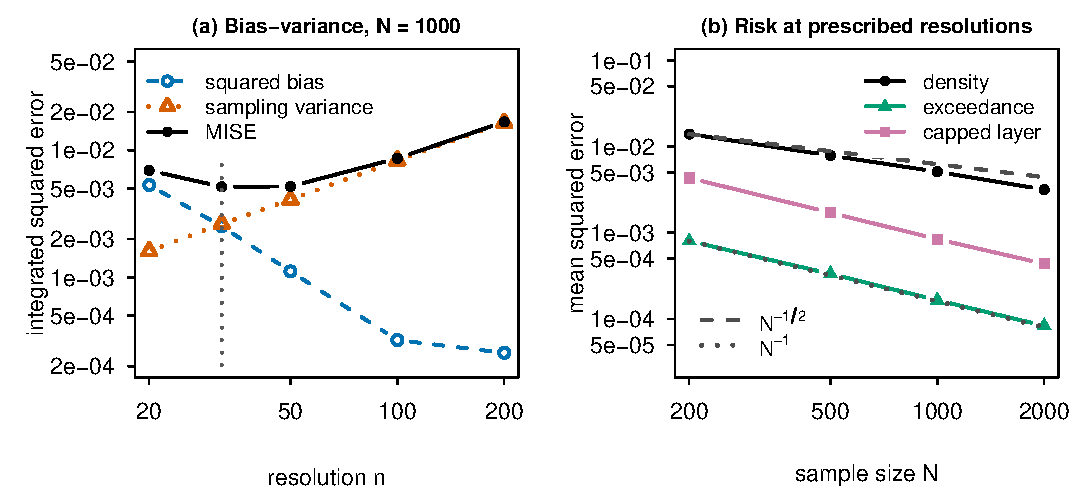
\includegraphics[width=\linewidth]{figures/numerical_demonstration.pdf}
\caption{Monte Carlo illustration of the derived inferential devices.
Panel (a) separates squared smoothing bias and sampling variance; the vertical
line is $\sqrt{1000}$.  Panel (b) uses the grid-selected $N^{1/2}$ density
resolutions for density loss and $n_{\Theta}=N$ for the two bounded
functionals.  The grey lines have the theoretical reference orders.}
\label{fig:numerical-demonstration}
\end{figure}

\begin{table}[!ht]
\centering
\color{blue}
\caption{Risk summary.  Functional entries are empirical RMSE, with mean
posterior standard deviation in parentheses.  $\overline K_D$ is the mean
number of occupied components at resolution $n_D$.}
\label{tab:numerical-demonstration}
\scriptsize
\setlength{\tabcolsep}{3.6pt}
\begin{tabular}{rrrrrr}
\toprule
$N$ & $n_D$ & $\overline K_D$ & Density MISE & Exceedance & Capped layer \\
\midrule
200  & 20 & 190  & 0.01289 & 0.02749 (0.02798) & 0.06408 (0.06484) \\
500  & 20 & 439  & 0.00821 & 0.01827 (0.01790) & 0.04141 (0.04115) \\
1000 & 50 & 957  & 0.00518 & 0.01277 (0.01276) & 0.02895 (0.02919) \\
2000 & 50 & 1836 & 0.00318 & 0.00910 (0.00905) & 0.02106 (0.02063) \\
\bottomrule
\end{tabular}
\end{table}

At $N=1000$, the density MISE among the regular candidates was minimized at
$n=50$; the values $20$ and $50$ bracket $\sqrt{1000}\simeq32$.  Increasing
$n$ over the candidate grid reduced squared smoothing bias but increased
sampling variation and the occupied-component count.  The Monte
Carlo integrated posterior loss agreed with the empirical counterpart of
\eqref{eq:integrated-posterior-local-risk-exact} to within $2.8\%$ across the
four sample sizes.  The descriptive log--log slopes were $-0.61$ for density
MISE and $-0.96$ and $-0.97$ for the MSEs of the two functionals, compared
with the respective reference orders $N^{-1/2}$ and $N^{-1}$.  The posterior standard deviations
in Table~\ref{tab:numerical-demonstration} also track the repeated-sampling
RMSEs.  For example, at $N=1000$ the mean posterior covariance between the two
valuations was $3.44\times10^{-4}$, compared with an empirical covariance of
$3.37\times10^{-4}$.  These finite-sample comparisons are descriptive rather
than additional asymptotic or coverage claims.

The experiment demonstrates the Bayesian-bootstrap construction studied here;
it does not assess an adaptive or EM fit, an uncapped stop loss, or frequentist
coverage of posterior credible sets.  All code, parameter settings, random
seeds, reference calculations, and files reproducing
Figure~\ref{fig:numerical-demonstration} and
Table~\ref{tab:numerical-demonstration} are available at
\url{https://github.com/hiendn/multivariate-erlang-mixture-inference}.
\end{revision}

\section{Discussion}
\label{sec:discussion}

\begin{revision}
The approximation operator supplies the smoothing bias of a fitted
Bayesian-bootstrap Erlang mixture.  Together with the kernel norm bound and
Dirichlet variance identity, it gives local density-risk bounds and risk
bounds for bounded actuarial valuations.  The fixed-grid transfer inequality
also separates operator bias from errors in other estimates of the cell
weights.  Any application to such estimates needs a corresponding statistical
bound for those weight errors.

The examples in \cite{LeeLin2012} illustrate both the reach and the
limits of these results.  Their twelve-dimensional lognormal example has a
bounded, Lipschitz density and a finite inverse half-moment, as verified for
nonsingular lognormal laws in Lemma~\ref{lem:inverse-half-moment-check}.
For data from this model, Corollary~\ref{cor:minimax-local-density} with
$d=12$ and $\alpha=1$ gives the upper rate $N^{-1/7}$ for local squared
density error of the smoothed Bayesian-bootstrap estimator.  The bounded
aggregate valuations in Corollary~\ref{cor:closed-form-actuarial} instead have
squared-error order $N^{-1}$ when $n\asymp N$.  This comparison distinguishes
the dimension-dependent density-risk bound from the bound for a fixed capped
valuation.  The numerical accuracy of their EM fit is a separate question. 

Their bivariate extreme-dependence examples start from the upper and lower
Fr\'echet--Hoeffding couplings of continuous gamma marginals.  Those target
laws are supported on curves and have no bivariate Lebesgue density.  The
measure-smoothing construction in Proposition~\ref{prop:measure-smoothing-transfer}
is still defined, but the density-approximation and density-risk theorems do
not apply to those singular targets.  Thus weak approximation of a joint law
and approximation of its density answer different questions in these
examples.

The valuation results also apply beyond insurance to bounded reliability or
risk indicators whose nonconstant part has compact support.

Other uses of the approximation bounds need not employ the Bayesian bootstrap.
For a fixed dictionary, likelihood or other weight estimators could be studied
by combining Proposition~\ref{prop:measure-smoothing-transfer} with their
weight-error bounds.  Methods that select the shapes, common rate, or penalty
require additional control of that selection step.  Extending this analysis
to the censored-data setting of \cite{VerbelenAntonioClaeskens2016} would also
require a sampling model that accounts for censoring rather than treating
censored observations as complete losses.

Further questions concern data-driven resolution selection and posterior
credible-interval coverage.  The present risk calculations suggest how to
balance smoothing and sampling error, but do not establish adaptation to
unknown smoothness or a Bernstein--von Mises limit.  Extending the valuation results to unbounded valuations
would require the additional tail control identified after
Corollary~\ref{cor:closed-form-actuarial}.
\end{revision}

\appendix
\section{Additional weighted and component-count approximation results}
\label{app:additional-approximation}

\subsection{Weighted qualitative and scale results}
We now consider qualitative approximation in weighted sup norms.

\begin{theorem}[Qualitative convergence in $L_{\infty,\nu}$]\label{thm:weighted-qualitative}
Let $\nu\ge0$ and let $f\in L_{\infty,\nu}(\mathbb{R}_{+}^{d})$.
Assume that 
\begin{equation}
\Omega_{\nu,*}(f;\delta)\longrightarrow0\qquad(\delta\downarrow0).\label{eq:intrinsic-modulus-zero-main}
\end{equation}
Then 
\[
\left\lVert \mathcal{K}_{n}^{(d)}f-f\right\rVert _{\infty,\nu}\longrightarrow0\qquad(n\to\infty).
\]
More quantitatively, for every $\delta>0$ and every $n\in\mathbb{N}$,
\begin{equation}
\left\lVert \mathcal{K}_{n}^{(d)}f-f\right\rVert _{\infty,\nu}\le\Omega_{\nu,*}(f;\delta)+\left\lVert f\right\rVert _{\infty,\nu}\left(\frac{1+d/3}{n\delta^{2}}+\frac{\sqrt{A_{2\nu,d}(1+d/3)}}{\sqrt{n}\,\delta}\right),\label{eq:qualitative-weighted-estimate-main}
\end{equation}
where $A_{2\nu,d}$ is the constant from Lemma~\ref{lem:weighted-moments}
at the index $2\nu$. \end{theorem}

\begin{corollary}[Uniform convergence on $C_{0}$]\label{cor:global-uniform-c0}
Let $f\in C_{0}(\mathbb{R}_{+}^{d})$. Then 
\[
\left\lVert \mathcal{K}_{n}^{(d)}f-f\right\rVert _{L^{\infty}(\mathbb{R}_{+}^{d})}\longrightarrow0\qquad(n\to\infty).
\]
If, in addition, $[f]_{0,\alpha,*}<\infty$ for some $0<\alpha\le1$,
then 
\[
\left\lVert \mathcal{K}_{n}^{(d)}f-f\right\rVert _{L^{\infty}(\mathbb{R}_{+}^{d})}\le C_{\alpha,d}[f]_{0,\alpha,*}\,n^{-\alpha/2}\qquad(n\in\mathbb{N}),
\]
where one may take $C_{\alpha,d}=(1+d/3)^{\alpha/2}$. The same qualitative
conclusion also holds for every bounded continuous $f$ such that
$f-L\in C_{0}(\mathbb{R}_{+}^{d})$ for some constant $L\in\mathbb{R}$.
\end{corollary}

\begin{corollary}[Finite Erlang mixture approximation in weighted
sup norms]\label{cor:weighted-finite} Let $\nu\ge0$, and let $f\in\mathcal{D}_{1}(\mathbb{R}_{+}^{d})\cap L_{\infty,\nu}(\mathbb{R}_{+}^{d})$.
Suppose that $\mathcal{K}_{n}^{(d)}f\to f$ in $L_{\infty,\nu}(\mathbb{R}_{+}^{d})$. Then there exists
a sequence $(g_{n})_{n\ge1}$ of finite multivariate Erlang mixture
densities with common scale parameter $1/n$ such that 
\[
\left\lVert g_{n}-f\right\rVert _{\infty,\nu}\longrightarrow0.
\]
\end{corollary}

The next pair of theorems give global weighted sup-norm and $L^p$ rates.

\begin{theorem}[Weighted H\"older rate in $L_{\infty,\nu}$]\label{thm:weighted-holder-rate}
Let $\nu\ge0$ and $0<\alpha\le1$. If $f\in L_{\infty,\nu}(\mathbb{R}_{+}^{d})$
and $[f]_{\nu,\alpha,*}<\infty$, then for every $n\in\mathbb{N}$,
\begin{equation}
\left\lVert \mathcal{K}_{n}^{(d)}f-f\right\rVert _{\infty,\nu}\le C_{\alpha,d}[f]_{\nu,\alpha,*}\,n^{-\alpha/2},\label{eq:weighted-holder-rate-main}
\end{equation}
where one may take $C_{\alpha,d}=(1+d/3)^{\alpha/2}$. \end{theorem}

\begin{theorem}[Weighted $L^p$ rate from an integrated intrinsic H\"older envelope]\label{thm:weighted-lp-rate}
Let $1\le p<\infty$, let $\eta\ge0$, let $0<\alpha\le1$, and let
$f:\mathbb{R}_{+}^{d}\to\mathbb{R}$ be measurable. Assume that there
exists a measurable function $H\in L_{p,\eta}(\mathbb{R}_{+}^{d})$
such that 
\begin{equation}
\left\lvert f(y)-f(x)\right\rvert \le H(x)\left(\frac{\left\lVert y-x\right\rVert _{2}}{\sqrt{1+\left\lVert x\right\rVert _{1}}}\right)^{\alpha}\qquad(x,y\in\mathbb{R}_{+}^{d}).\label{eq:weighted-lp-envelope-main}
\end{equation}
Then, for every $n\in\mathbb{N}$, 
\begin{equation}
\left\lVert \mathcal{K}_{n}^{(d)}f-f\right\rVert _{p,\eta}\le C_{\alpha,d}\,n^{-\alpha/2}\,\left\lVert H\right\rVert _{p,\eta},\label{eq:weighted-lp-rate-main}
\end{equation}
where one may take $C_{\alpha,d}=(1+d/3)^{\alpha/2}$. \end{theorem}

\begin{corollary}[From weighted sup-norm control to weighted $L^{p}$
control]\label{cor:weighted-sup-to-lp} Let $1\le p<\infty$, let
$\nu\ge0$, let $0<\alpha\le1$, and let $\eta>\nu p+d$. Suppose
that $f\in L_{\infty,\nu}(\mathbb{R}_{+}^{d})$ and $[f]_{\nu,\alpha,*}<\infty$.
Then 
\begin{equation}
\left\lVert \mathcal{K}_{n}^{(d)}f-f\right\rVert _{p,\eta}\le C_{\alpha,d}\,B_{p,\eta,\nu,d}\,[f]_{\nu,\alpha,*}\,n^{-\alpha/2},\label{eq:weighted-sup-to-lp-main}
\end{equation}
where 
\[
B_{p,\eta,\nu,d}=\left(\int_{\mathbb{R}_{+}^{d}}(1+\left\lVert x\right\rVert _{1})^{\nu p-\eta}\,\mathrm{d}x\right)^{1/p}<\infty.
\]
In particular, $\left\lVert \mathcal{K}_{n}^{(d)}f-f\right\rVert _{p,\eta}=O(n^{-\alpha/2})$.
\end{corollary}

\begin{remark}[Unweighted $L^{p}$ rates]\label{rem:unweighted-lp}
Taking $\eta=0$ in Theorem~\ref{thm:weighted-lp-rate} yields the
ordinary unweighted estimate 
\[
\left\lVert \mathcal{K}_{n}^{(d)}f-f\right\rVert _{L^{p}(\mathbb{R}_{+}^{d})}\le C_{\alpha,d}\,n^{-\alpha/2}\,\left\lVert H\right\rVert _{L^{p}(\mathbb{R}_{+}^{d})}
\]
whenever $H\in L^{p}(\mathbb{R}_{+}^{d})$ satisfies \eqref{eq:weighted-lp-envelope-main}.
\textcolor{blue}{The estimate above is a sufficient bound under
\eqref{eq:weighted-lp-envelope-main}.  For $d=1$ and $1<p<\infty$,
\cite[Theorems~1--2]{Totik1983} characterizes $L^p$ approximation orders by
difference conditions and characterizes order $n^{-1}$ by a derivative
condition.  The present bound does not give a converse characterization.} \end{remark}

\subsection{Finite-mixture rates in the number of components}

\label{sec:component-rates}

We now pass from scale-dependent rates for the countable Erlang mixture
operator to explicit rates for finite mixtures indexed by the number
of components.

\begin{proposition}[Compact-set truncation]\label{prop:compact-tailfree}
Let $d\in\mathbb{N}$, let $M>0$, and let $f\in\mathcal{D}_{1}(\mathbb{R}_{+}^{d})$.
Write 
\[
\mathcal{K}_{n}^{(d)}f=\sum_{m\in\mathbb{N}^{d}}a_{m,n}\,\varphi_{m,n},\qquad\varphi_{m,n}(x)=\prod_{j=1}^{d}\tau_{m_{j},n}(x_{j}).
\]
For $J\in\mathbb{N}$ with $J\ge nM$, define 
\[
F_{J}=\{m\in\mathbb{N}^{d}:1\le m_{j}\le J\text{ for all }j=1,\dots,d\},\qquad r_{n,J}=\sum_{m\notin F_{J}}a_{m,n},
\]
set $\ell_{J}=(J+1,\dots,J+1)\in\mathbb{N}^{d}$, and define 
\[
\widetilde{g}_{n,J}^{(M)}=\sum_{m\in F_{J}}a_{m,n}\,\varphi_{m,n}+r_{n,J}\,\varphi_{\ell_{J},n}.
\]
Then $\widetilde{g}_{n,J}^{(M)}$ is a finite multivariate Erlang
mixture density with at most $J^{d}+1$ components, and 
\begin{equation}
\left\lVert \mathcal{K}_{n}^{(d)}f-\widetilde{g}_{n,J}^{(M)}\right\rVert _{L^{\infty}(Q_{M})}\le2n^{d}e^{-nM}\frac{(nM)^{J}}{J!}.\label{eq:compact-tailfree-trunc-main}
\end{equation}
If, in addition, $f$ is bounded and continuous on $\mathbb{R}_{+}^{d}$,
then for every $r>0$, 
\begin{align}
\left\lVert \widetilde{g}_{n,J}^{(M)}-f\right\rVert _{L^{\infty}(Q_{M})} & \le\omega_{Q_{M+r}}(f;r)+\frac{2\left\lVert f\right\rVert _{L^{\infty}(\mathbb{R}_{+}^{d})}}{r^{2}}\left(\frac{dM}{n}+\frac{d}{3n^{2}}\right)\nonumber \\
 & \qquad+2n^{d}e^{-nM}\frac{(nM)^{J}}{J!}.\label{eq:compact-tailfree-modulus-main}
\end{align}
\end{proposition}

\begin{corollary}[Component-count compact-set rate]\label{cor:compact-component-rate}
Let $d\in\mathbb{N}$, let $M>0$, let $0<\alpha\le1$, and let $f\in\mathcal{D}_{1}(\mathbb{R}_{+}^{d})\cap L^{\infty}(\mathbb{R}_{+}^{d})$.
Assume that there is a constant $H>0$ such that 
\[
\left\lvert f(y)-f(z)\right\rvert \le H\left\lVert y-z\right\rVert _{2}^{\alpha}\qquad(y,z\in Q_{M+1}).
\]
Then there exist constants $C>0$ and $K_{0}\in\mathbb{N}$ such that
for every integer $K\ge K_{0}$ there exists a finite multivariate
Erlang mixture density $g_{K}$ with at most $K$ components and 
\[
\left\lVert g_{K}-f\right\rVert _{L^{\infty}(Q_{M})}\le CK^{-\alpha/(2d)}.
\]
\end{corollary}

To obtain a global weighted sup-norm component-count rate, we require the following
shape-decay bound for Erlang kernels.

\begin{lemma}[Shape decay of Erlang kernels in sup norm]\label{lem:erlang-shape-sup}
For every $m,n\in\mathbb{N}$, 
\[
\left\lVert \tau_{m,n}\right\rVert _{L^{\infty}(\mathbb{R}_{+})}\le nm^{-1/2}.
\]
Consequently, if $m=(m_{1},\dots,m_{d})\in\mathbb{N}^{d}$ has some
coordinate $m_{j}\ge J+1$, then for every $\nu\ge0$, 
\[
\left\lVert \varphi_{m,n}\right\rVert _{\infty,\nu}\le n^{d}(J+1)^{-1/2}.
\]
\end{lemma}

\begin{proposition}[Truncation in weighted sup norms]\label{prop:weighted-tailfree}
Let $d\in\mathbb{N}$, let $\nu\ge0$, and let $f\in\mathcal{D}_{1}(\mathbb{R}_{+}^{d})$.
Write 
\[
\mathcal{K}_{n}^{(d)}f=\sum_{m\in\mathbb{N}^{d}}a_{m,n}\,\varphi_{m,n}.
\]
For $J\in\mathbb{N}$, define 
\[
F_{J}=\{m\in\mathbb{N}^{d}:1\le m_{j}\le J\text{ for all }j=1,\dots,d\},\qquad r_{n,J}=\sum_{m\notin F_{J}}a_{m,n},
\]
set $\ell_{J}=(J+1,\dots,J+1)$, and define 
\[
\widetilde{g}_{n,J}^{(\nu)}=\sum_{m\in F_{J}}a_{m,n}\,\varphi_{m,n}+r_{n,J}\,\varphi_{\ell_{J},n}.
\]
Then $\widetilde{g}_{n,J}^{(\nu)}$ is a finite multivariate Erlang
mixture density with at most $J^{d}+1$ components, and 
\begin{equation}
\left\lVert \mathcal{K}_{n}^{(d)}f-\widetilde{g}_{n,J}^{(\nu)}\right\rVert _{\infty,\nu}\le2n^{d}(J+1)^{-1/2}.\label{eq:weighted-tailfree-trunc-main}
\end{equation}
\end{proposition}

\begin{corollary}[Component-count rate for weighted sup norms]\label{cor:weighted-component-rate}
Let $d\in\mathbb{N}$, let $\nu\ge0$, let $0<\alpha\le1$, and let
$f\in\mathcal{D}_{1}(\mathbb{R}_{+}^{d})\cap L_{\infty,\nu}(\mathbb{R}_{+}^{d})$.
Assume that $[f]_{\nu,\alpha,*}<\infty$. Then there exist constants
$C>0$ and $K_{0}\in\mathbb{N}$ such that for every integer $K\ge K_{0}$
there exists a finite multivariate Erlang mixture density $g_{K}$
with at most $K$ components and 
\[
\left\lVert g_{K}-f\right\rVert _{\infty,\nu}\le CK^{-\alpha/[2d(2d+\alpha)]}.
\]
 \end{corollary}

The same truncation idea also yields component-count
rates in weighted $L^{p}$ norms for $1<p<\infty$.

\begin{lemma}[Shape decay of Erlang kernels in $L^{p}$]\label{lem:erlang-shape-lp}
Let $1<p<\infty$. Then, for every $m,n\in\mathbb{N}$, 
\[
\left\lVert \tau_{m,n}\right\rVert _{L^{p}(\mathbb{R}_{+})}\le n^{1-1/p}m^{-(1-1/p)/2}.
\]
Consequently, if $m=(m_{1},\dots,m_{d})\in\mathbb{N}^{d}$ has some
coordinate $m_{j}\ge J+1$, then for every $\eta\ge0$, 
\[
\left\lVert \varphi_{m,n}\right\rVert _{p,\eta}\le n^{d(1-1/p)}(J+1)^{-(1-1/p)/2}.
\]
\end{lemma}

\begin{proposition}[Truncation in weighted $L^{p}$ norms]\label{prop:weighted-lp-tailfree}
Let $d\in\mathbb{N}$, let $1<p<\infty$, let $\eta\ge0$, and let
$f\in\mathcal{D}_{1}(\mathbb{R}_{+}^{d})$. Write 
\[
\mathcal{K}_{n}^{(d)}f=\sum_{m\in\mathbb{N}^{d}}a_{m,n}\,\varphi_{m,n}.
\]
For $J\in\mathbb{N}$, define 
\[
F_{J}=\{m\in\mathbb{N}^{d}:1\le m_{j}\le J\text{ for all }j=1,\dots,d\},\qquad r_{n,J}=\sum_{m\notin F_{J}}a_{m,n},
\]
set $\ell_{J}=(J+1,\dots,J+1)$, and define 
\[
\widetilde{g}_{n,J}^{(p,\eta)}=\sum_{m\in F_{J}}a_{m,n}\,\varphi_{m,n}+r_{n,J}\,\varphi_{\ell_{J},n}.
\]
Then $\widetilde{g}_{n,J}^{(p,\eta)}$ is a finite multivariate Erlang
mixture density with at most $J^{d}+1$ components, and 
\begin{equation}
\left\lVert \mathcal{K}_{n}^{(d)}f-\widetilde{g}_{n,J}^{(p,\eta)}\right\rVert _{p,\eta}\le2n^{d(1-1/p)}(J+1)^{-(1-1/p)/2}.\label{eq:weighted-lp-tailfree-trunc-main}
\end{equation}
\end{proposition}

\begin{corollary}[Component-count rate in weighted $L^{p}$ norms]\label{cor:weighted-lp-component-rate}
Let $d\in\mathbb{N}$, let $1<p<\infty$, let $\eta\ge0$, let $0<\alpha\le1$,
and let $f\in\mathcal{D}_{1}(\mathbb{R}_{+}^{d})$. Assume that there
exists a measurable function $H\in L_{p,\eta}(\mathbb{R}_{+}^{d})$
such that 
\[
\left\lvert f(y)-f(x)\right\rvert \le H(x)\left(\frac{\left\lVert y-x\right\rVert _{2}}{\sqrt{1+\left\lVert x\right\rVert _{1}}}\right)^{\alpha}\qquad(x,y\in\mathbb{R}_{+}^{d}).
\]
Then there exist constants $C>0$ and $K_{0}\in\mathbb{N}$ such that
for every integer $K\ge K_{0}$ there exists a finite multivariate
Erlang mixture density $g_{K}$ with at most $K$ components and 
\[
\left\lVert g_{K}-f\right\rVert _{p,\eta}\le CK^{-\alpha/[2d(2d+\alpha p/(p-1))]}.
\]
\end{corollary}

\begin{remark}\label{rem:component-rate-remarks} \textcolor{blue}{The compact-set bound in Corollary~\ref{cor:compact-component-rate}
has a larger component-count exponent because its proof chooses
$J_n=\lceil n(M+1)\rceil$, which makes the truncation factor
$e^{-nM}(nM)^{J_n}/J_n!$ exponentially small in $n$.
The global weighted bounds use algebraic shape decay and have smaller
component-count exponents under their respective assumptions.} Corollary~\ref{cor:weighted-component-rate}
\textcolor{blue}{has the exponent obtained from Corollary~\ref{cor:weighted-lp-component-rate}
in the limit $p\to\infty$.}
By contrast, this truncation strategy does not yield a component-count
rate in ordinary unweighted $L^{1}$, because every Erlang density
has $L^{1}$ norm equal to $1$, independently of its shape. \end{remark}

\section{Proofs of the approximation results}

\label{sec:proofs}

\subsection{One-dimensional input, tensorization, and qualitative approximation}

The next two lemmas transfer the one-dimensional $L^{p}$ approximation
property to the coordinatewise lifted operators.

\begin{lemma}[Coordinatewise $L^{p}$ contraction]\label{lem:coord-contraction}
Let $1\le p<\infty$, $n\in\mathbb{N}$, and $j\in\{1,\dots,d\}$.
Then $K_{n,j}$ maps $L^{p}(\mathbb{R}_{+}^{d})$ into itself and
\[
\left\lVert K_{n,j}f\right\rVert _{L^{p}(\mathbb{R}_{+}^{d})}\le\left\lVert f\right\rVert _{L^{p}(\mathbb{R}_{+}^{d})}\qquad(f\in L^{p}(\mathbb{R}_{+}^{d})).
\]
In particular, each $K_{n,j}$ is a positive linear contraction on
$L^{p}(\mathbb{R}_{+}^{d})$. \end{lemma}

\begin{lemma}[Coordinatewise convergence]\label{lem:coord-convergence}
Let $1\le p<\infty$ and $j\in\{1,\dots,d\}$. Then, for every $f\in L^{p}(\mathbb{R}_{+}^{d})$,
\[
\left\lVert K_{n,j}f-f\right\rVert _{L^{p}(\mathbb{R}_{+}^{d})}\longrightarrow0\qquad(n\to\infty).
\]
\end{lemma}

\begin{lemma}[Uniform $L^{p}$ bound for Erlang kernels]\label{lem:kernel-bound}
Let $1\le p<\infty$ and $m,n\in\mathbb{N}$. Then
\[
0\le\tau_{m,n}(x)\le n\qquad(x\ge0),
\]
and therefore 
\[
\left\lVert \tau_{m,n}\right\rVert _{L^{p}(\mathbb{R}_{+})}\le n^{1-1/p}.
\]
Consequently, for every $m=(m_{1},\dots,m_{d})\in\mathbb{N}^{d}$,
\begin{equation}
\left\|\prod_{j=1}^{d}\tau_{m_{j},n}(\cdot_{j})\right\|_{L^{p}(\mathbb{R}_{+}^{d})}\le n^{d(1-1/p)}.\label{eq:product-bound-main}
\end{equation}
\end{lemma} 
\begin{proof}[Proof of Theorem~\ref{thm:1d-input}]
The positivity and linearity are immediate from \eqref{eq:Kn-def-main}.
For the contraction property, write 
\[
p_{n,k}(x)=e^{-nx}\frac{(nx)^{k}}{k!},\qquad I_{k}=\left[\frac{k}{n},\frac{k+1}{n}\right),\qquad k\in\mathbb{N}_{0}.
\]
Since $\sum_{k=0}^{\infty}p_{n,k}(x)=1$, Jensen's inequality and then
Jensen's inequality on each interval $I_{k}$ with respect to the probability
measure $n\,\mathrm{d}t$ give 
\begin{align*}
|K_{n}g(x)|^{p} & \le\sum_{k=0}^{\infty}p_{n,k}(x)\left(n\int_{I_{k}}|g(t)|\,\mathrm{d}t\right)^{p}\\
 & \le\sum_{k=0}^{\infty}p_{n,k}(x)\,n\int_{I_{k}}|g(t)|^{p}\,\mathrm{d}t.
\end{align*}
Integrating over $x\in\mathbb{R}_{+}$ and using Tonelli's theorem, we obtain
\begin{align*}
\|K_{n}g\|_{L^{p}(\mathbb{R}_{+})}^{p} & \le\sum_{k=0}^{\infty}\left(\int_{0}^{\infty}p_{n,k}(x)\,\mathrm{d}x\right)\,n\int_{I_{k}}|g(t)|^{p}\,\mathrm{d}t\\
 & =\sum_{k=0}^{\infty}\int_{I_{k}}|g(t)|^{p}\,\mathrm{d}t=\|g\|_{L^{p}(\mathbb{R}_{+})}^{p},
\end{align*}
because $\int_{0}^{\infty}p_{n,k}(x)\,\mathrm{d}x=1/n$. Thus $K_{n}$ is a positive
linear contraction on $L^{p}(\mathbb{R}_{+})$. The remaining strong $L^{p}$
convergence assertion is exactly Theorem~3.5 of
\cite{AltomareCappellettiLeonessa2013}, specialized to the choice
$a_{n}=0$ and $b_{n}=1$, for which the generalized operators in that
paper coincide with $K_{n}$. This proves the theorem. 
\end{proof}
%
\begin{proof}[Proof of Proposition~\ref{prop:1d-representation}]
The positivity of the coefficients in \eqref{eq:1d-cell-mass} is
immediate. Since the intervals $[(m-1)/n,m/n)$ partition $\mathbb{R}_{+}$
up to endpoints, 
\[
\sum_{m=1}^{\infty}a_{m,n}=\sum_{m=1}^{\infty}\int_{(m-1)/n}^{m/n}f(t)\,\mathrm{d}t=\int_{0}^{\infty}f(t)\,\mathrm{d}t=1.
\]
Re-indexing \eqref{eq:Kn-def-main} with $m=k+1$ gives 
\begin{align*}
(K_{n}f)(x) & =n\sum_{k=0}^{\infty}e^{-nx}\frac{(nx)^{k}}{k!}\int_{k/n}^{(k+1)/n}f(t)\,\mathrm{d}t\\
 & =\sum_{m=1}^{\infty}\left(\int_{(m-1)/n}^{m/n}f(t)\,\mathrm{d}t\right)ne^{-nx}\frac{(nx)^{m-1}}{(m-1)!}\\
 & =\sum_{m=1}^{\infty}a_{m,n}\,\tau_{m,n}(x),
\end{align*}
which is exactly \eqref{eq:1d-mixed-erlang-representation}. 
\end{proof}
%
\begin{proof}[Proof of Lemma~\ref{lem:coord-contraction}]
Fix $f\in L^{p}(\mathbb{R}_{+}^{d})$. By Fubini's theorem, for almost
every $x_{-j}\in\mathbb{R}_{+}^{d-1}$ the slice $f_{x_{-j}}(t)=f(x_{1},\dots,x_{j-1},t,x_{j+1},\dots,x_{d})$
belongs to $L^{p}(\mathbb{R}_{+})$. For such $x_{-j}$ we have $(K_{n,j}f)_{x_{-j}}=K_{n}(f_{x_{-j}})$.
Theorem~\ref{thm:1d-input} therefore gives 
\[
\int_{0}^{\infty}\left\lvert (K_{n,j}f)(x_{j},x_{-j})\right\rvert ^{p}\,\mathrm{d}x_{j}=\left\lVert K_{n}(f_{x_{-j}})\right\rVert _{L^{p}(\mathbb{R}_{+})}^{p}\le\left\lVert f_{x_{-j}}\right\rVert _{L^{p}(\mathbb{R}_{+})}^{p}.
\]
Integrating with respect to $x_{-j}$ and using Fubini's theorem once more yields
\begin{align*}
\left\lVert K_{n,j}f\right\rVert _{L^{p}(\mathbb{R}_{+}^{d})}^{p} & =\int_{\mathbb{R}_{+}^{d-1}}\int_{0}^{\infty}\left\lvert (K_{n,j}f)(x_{j},x_{-j})\right\rvert ^{p}\,\mathrm{d}x_{j}\,\mathrm{d}x_{-j}\\
 & \le\int_{\mathbb{R}_{+}^{d-1}}\int_{0}^{\infty}\left\lvert f(x_{j},x_{-j})\right\rvert ^{p}\,\mathrm{d}x_{j}\,\mathrm{d}x_{-j}=\left\lVert f\right\rVert _{L^{p}(\mathbb{R}_{+}^{d})}^{p}.
\end{align*}
The positivity and linearity are immediate from \eqref{eq:Knj-def-main}. 
\end{proof}
%
\begin{proof}[Proof of Lemma~\ref{lem:coord-convergence}]
Fix $f\in L^{p}(\mathbb{R}_{+}^{d})$ and $j\in\{1,\dots,d\}$. For
almost every $x_{-j}$ we again have $f_{x_{-j}}\in L^{p}(\mathbb{R}_{+})$
and $(K_{n,j}f)_{x_{-j}}=K_{n}(f_{x_{-j}})$. Therefore, by Theorem~\ref{thm:1d-input},
\[
\left\lVert K_{n}(f_{x_{-j}})-f_{x_{-j}}\right\rVert _{L^{p}(\mathbb{R}_{+})}\longrightarrow0\qquad(n\to\infty)
\]
for almost every $x_{-j}$. To pass to the outer integral, note that
the contraction property gives 
\begin{align*}
\left\lVert K_{n}(f_{x_{-j}})-f_{x_{-j}}\right\rVert _{L^{p}(\mathbb{R}_{+})}^{p} & \le2^{p-1}\left(\left\lVert K_{n}(f_{x_{-j}})\right\rVert _{L^{p}(\mathbb{R}_{+})}^{p}+\left\lVert f_{x_{-j}}\right\rVert _{L^{p}(\mathbb{R}_{+})}^{p}\right)\\
 & \le2^{p}\left\lVert f_{x_{-j}}\right\rVert _{L^{p}(\mathbb{R}_{+})}^{p}.
\end{align*}
The function $x_{-j}\mapsto\left\lVert f_{x_{-j}}\right\rVert _{L^{p}(\mathbb{R}_{+})}^{p}$
is integrable by Fubini's theorem, so dominated convergence yields 
\[
\left\lVert K_{n,j}f-f\right\rVert _{L^{p}(\mathbb{R}_{+}^{d})}^{p}=\int_{\mathbb{R}_{+}^{d-1}}\left\lVert K_{n}(f_{x_{-j}})-f_{x_{-j}}\right\rVert _{L^{p}(\mathbb{R}_{+})}^{p}\,\mathrm{d}x_{-j}\longrightarrow0.
\]
\end{proof}
%
\begin{proof}[Proof of Theorem~\ref{thm:tensor-convergence}]
By Lemma~\ref{lem:coord-contraction}, each $K_{n,j}$ is a positive
linear contraction on $L^{p}(\mathbb{R}_{+}^{d})$, hence so is their
composition $\mathcal{K}_{n}^{(d)}$. For convergence, write the telescoping
identity 
\begin{align*}
\mathcal{K}_{n}^{(d)}-I & =K_{n,1}\cdots K_{n,d}-I\\
 & =K_{n,1}\cdots K_{n,d-1}(K_{n,d}-I)+K_{n,1}\cdots K_{n,d-2}(K_{n,d-1}-I)+\cdots+(K_{n,1}-I).
\end{align*}
Applying this to $f$ and using that every preceding product is a
contraction, we obtain 
\begin{align*}
\left\lVert \mathcal{K}_{n}^{(d)}f-f\right\rVert _{L^{p}} & \le\sum_{j=1}^{d}\left\lVert K_{n,j}f-f\right\rVert _{L^{p}}.
\end{align*}
Each term on the right tends to $0$ by Lemma~\ref{lem:coord-convergence},
and the result follows. 
\end{proof}
%
\begin{proof}[Proof of Proposition~\ref{prop:explicit-mixed-erlang}]
The coefficients in \eqref{eq:cell-masses-main} are nonnegative
because $f\ge0$ a.e. Since the rectangles $\textcolor{blue}{\mathcal C_{m,n}}$ partition $\mathbb{R}_{+}^{d}$
up to boundaries, $\sum_{m\in\mathbb{N}^{d}}a_{m,n}=\sum_{m\in\mathbb{N}^{d}}\int_{\textcolor{blue}{\mathcal C_{m,n}}}f(t)\,\mathrm{d}t=\int_{\mathbb{R}_{+}^{d}}f(t)\,\mathrm{d}t=1$.
A repeated application of Tonelli's theorem shows that 
\begin{align*}
(\mathcal{K}_{n}^{(d)}f)(x) & =n^{d}\sum_{k\in\mathbb{N}_{0}^{d}}\left(\prod_{j=1}^{d}e^{-nx_{j}}\frac{(nx_{j})^{k_{j}}}{k_{j}!}\right)\int_{\prod_{j=1}^{d}[k_{j}/n,(k_{j}+1)/n)}f(t)\,\mathrm{d}t.
\end{align*}
Substituting $m_{j}=k_{j}+1$ for each coordinate transforms the cell
into $\textcolor{blue}{\mathcal C_{m,n}}$ and the product factor into $n^{d}\prod_{j=1}^{d}e^{-nx_{j}}\frac{(nx_{j})^{k_{j}}}{k_{j}!}=\prod_{j=1}^{d}ne^{-nx_{j}}\frac{(nx_{j})^{m_{j}-1}}{(m_{j}-1)!}=\prod_{j=1}^{d}\tau_{m_{j},n}(x_{j})$.
This proves \eqref{eq:multivariate-representation-main}. 
\end{proof}
%
\begin{proof}[Proof of Corollary~\ref{cor:countable}]
Combine Theorem~\ref{thm:tensor-convergence} with Proposition~\ref{prop:explicit-mixed-erlang}. 
\end{proof}
%
\begin{proof}[Proof of Corollary~\ref{cor:compact-finite}]
If some coordinate $m_{j}$ satisfies $m_{j}\ge\lfloor nM\rfloor+2$,
then the interval $[(m_{j}-1)/n,m_{j}/n)$ lies to the right of $M$,
so the cell $\textcolor{blue}{\mathcal C_{m,n}}$ is disjoint from $Q_{M}$ in the $j$th coordinate.
Since $f$ vanishes a.e.\ outside $Q_{M}$, the corresponding coefficient
$a_{m,n}$ is zero. Therefore only finitely many indices can appear
in \eqref{eq:multivariate-representation-main}. 
\end{proof}
%
\begin{proof}[Proof of Lemma~\ref{lem:kernel-bound}]
Since $e^{y}=\sum_{r=0}^{\infty}y^{r}/r!\ge y^{m-1}/(m-1)!$ for
$y\ge0$, we have $e^{-y}y^{m-1}/(m-1)!\le1$ for all $y\ge0$. Taking
$y=nx$ gives $\tau_{m,n}(x)\le n$, and therefore $\left\lVert \tau_{m,n}\right\rVert _{L^{p}(\mathbb{R}_{+})}^{p}=\int_{0}^{\infty}\tau_{m,n}(x)^{p}\,\mathrm{d}x\le n^{p-1}\int_{0}^{\infty}\tau_{m,n}(x)\,\mathrm{d}x=n^{p-1}$,
because $\tau_{m,n}$ is a probability density. This proves the one-dimensional
estimate. The product bound \eqref{eq:product-bound-main} follows
by Fubini's theorem. 
\end{proof}
%
\begin{proof}[Proof of Theorem~\ref{thm:finite-approx}]
Fix $f\in\mathcal{D}_{p}(\mathbb{R}_{+}^{d})$ and write $\mathcal{K}_{n}^{(d)}f=\sum_{m\in\mathbb{N}^{d}}a_{m,n}\,\varphi_{m,n}$,
where $\varphi_{m,n}(x)=\prod_{j=1}^{d}\tau_{m_{j},n}(x_{j})$. For
$N\in\mathbb{N}$, define the finite index set $F_{N}=\{m\in\mathbb{N}^{d}:1\le m_{j}\le N\text{ for all }j=1,\dots,d\}$
and the tail mass $r_{n,N}=\sum_{m\notin F_{N}}a_{m,n}$. Because
the coefficients are nonnegative and sum to $1$, we have $r_{n,N}\downarrow0$
as $N\to\infty$ for each fixed $n$. Define the finite mixture 
\begin{equation}
g_{n,N}=\sum_{m\in F_{N}}a_{m,n}\,\varphi_{m,n}+r_{n,N}\,\varphi_{\mathbf{1},n},\label{eq:gnN-main}
\end{equation}
where $\mathbf{1}=(1,\dots,1)\in\mathbb{N}^{d}$. Then $g_{n,N}$
is a finite multivariate Erlang mixture density.

Since $\mathcal{K}_{n}^{(d)}f-g_{n,N}=\sum_{m\notin F_{N}}a_{m,n}(\varphi_{m,n}-\varphi_{\mathbf{1},n})$,
Lemma~\ref{lem:kernel-bound} gives 
\begin{align*}
\left\lVert \mathcal{K}_{n}^{(d)}f-g_{n,N}\right\rVert _{L^{p}} & \le\sum_{m\notin F_{N}}a_{m,n}\left(\left\lVert \varphi_{m,n}\right\rVert _{L^{p}}+\left\lVert \varphi_{\mathbf{1},n}\right\rVert _{L^{p}}\right)\\
 & \le2n^{d(1-1/p)}\sum_{m\notin F_{N}}a_{m,n}=2n^{d(1-1/p)}r_{n,N}.
\end{align*}
For each fixed $n$, choose $N(n)$ so large that $\left\lVert \mathcal{K}_{n}^{(d)}f-g_{n,N(n)}\right\rVert _{L^{p}(\mathbb{R}_{+}^{d})}\le1/n$.
Set $g_{n}=g_{n,N(n)}$. Then each $g_{n}$ is a finite multivariate
Erlang mixture density with common scale $1/n$, and 
\begin{align*}
\left\lVert g_{n}-f\right\rVert _{L^{p}} & \le\left\lVert g_{n}-\mathcal{K}_{n}^{(d)}f\right\rVert _{L^{p}}+\left\lVert \mathcal{K}_{n}^{(d)}f-f\right\rVert _{L^{p}}\\
 & \le\frac{1}{n}+\left\lVert \mathcal{K}_{n}^{(d)}f-f\right\rVert _{L^{p}}\longrightarrow0
\end{align*}
by Theorem~\ref{thm:tensor-convergence}. 
\end{proof}
%
\begin{proof}[Proof of Theorem~\ref{thm:weighted-qualitative}]
Fix $x\in\mathbb{R}_{+}^{d}$ and write $Y=Y_{n,x}$ and $\Delta=Y-x$.
Let $A_{n,\delta}(x)=\{\left\lVert \Delta\right\rVert _{2}>\delta\sqrt{1+\left\lVert x\right\rVert _{1}}\}$.
Since $f\in L_{\infty,\nu}(\mathbb{R}_{+}^{d})$ and Lemma~\ref{lem:weighted-moments}
gives $\mathbb{E}[w_{\nu}(Y)]<\infty$, we have $\mathbb{E}[|f(Y)|]<\infty$.
Hence Proposition~\ref{prop:prob-representation} applies and $(\mathcal{K}_{n}^{(d)}f)(x)-f(x)=\mathbb{E}[f(Y)-f(x)]$.
On the near event $A_{n,\delta}(x)^{c}$, the definition of $\Omega_{\nu,*}(f;\delta)$
gives $\left\lvert f(Y)-f(x)\right\rvert /w_{\nu}(x)\le\Omega_{\nu,*}(f;\delta)$,
and therefore $\frac{1}{w_{\nu}(x)}\mathbb{E}\left[\left\lvert f(Y)-f(x)\right\rvert \mathbf{1}_{A_{n,\delta}(x)^{c}}\right]\le\Omega_{\nu,*}(f;\delta)$.
On the far event, the weighted norm gives $\left\lvert f(Y)-f(x)\right\rvert \le\left\lvert f(Y)\right\rvert +\left\lvert f(x)\right\rvert \le\left\lVert f\right\rVert _{\infty,\nu}\left(w_{\nu}(Y)+w_{\nu}(x)\right)$,
hence 
\begin{align*}
\frac{1}{w_{\nu}(x)}\mathbb{E}\left[\left\lvert f(Y)-f(x)\right\rvert \mathbf{1}_{A_{n,\delta}(x)}\right] & \le\left\lVert f\right\rVert _{\infty,\nu}\left(\mathbb{P}(A_{n,\delta}(x))+\frac{\mathbb{E}[w_{\nu}(Y)\mathbf{1}_{A_{n,\delta}(x)}]}{w_{\nu}(x)}\right).
\end{align*}
By Lemma~\ref{lem:displacement-moments}, 
\begin{align*}
\mathbb{P}(A_{n,\delta}(x)) & \le\frac{\mathbb{E}[\left\lVert \Delta\right\rVert _{2}^{2}]}{\delta^{2}(1+\left\lVert x\right\rVert _{1})}\le\frac{1+d/3}{n\delta^{2}}.
\end{align*}
For the weighted expectation term, Cauchy--Schwarz and Lemma~\ref{lem:weighted-moments}
at the index $2\nu$ yield 
\begin{align*}
\frac{\mathbb{E}[w_{\nu}(Y)\mathbf{1}_{A_{n,\delta}(x)}]}{w_{\nu}(x)} & \le\frac{\mathbb{E}[w_{2\nu}(Y)]^{1/2}}{w_{\nu}(x)}\,\mathbb{P}(A_{n,\delta}(x))^{1/2}\\
 & \le\sqrt{A_{2\nu,d}}\,\mathbb{P}(A_{n,\delta}(x))^{1/2}\\
 & \le\frac{\sqrt{A_{2\nu,d}(1+d/3)}}{\sqrt{n}\,\delta}.
\end{align*}
Combining the near- and far-event estimates proves \eqref{eq:qualitative-weighted-estimate-main}.
To obtain convergence, fix $\delta>0$ and let $n\to\infty$, then
let $\delta\downarrow0$ and use \eqref{eq:intrinsic-modulus-zero-main}. 
\end{proof}
%
\begin{proof}[Proof of Corollary~\ref{cor:global-uniform-c0}]
The rate bound is immediate from Theorem~\ref{thm:weighted-holder-rate}
with $\nu=0$. For the qualitative convergence, it is enough to verify
that $\Omega_{0,*}(f;\delta)\to0$ as $\delta\downarrow0$, because
then Theorem~\ref{thm:weighted-qualitative} applies with $\nu=0$.

Fix $\varepsilon>0$. Since $f\in C_{0}(\mathbb{R}_{+}^{d})$, there
exists $R>0$ such that 
\[
\left\lvert f(z)\right\rvert <\frac{\varepsilon}{4}\qquad\text{whenever }\left\lVert z\right\rVert _{1}\ge\frac{R}{2}.
\]
Increase $R$, if necessary, so that 
\[
\sqrt{d}\sqrt{1+s}\le\frac{s}{2}\qquad(s\ge R).
\]
Set 
\[
K=\left\{ z\in\mathbb{R}_{+}^{d}:\left\lVert z\right\rVert _{1}\le R+\sqrt{d}\sqrt{1+R}\right\}.
\]
This set is compact, so $f$ is uniformly continuous on $K$. Choose
$\eta>0$ such that 
\[
\left\lvert f(y)-f(x)\right\rvert <\frac{\varepsilon}{2}\qquad(x,y\in K,\ \left\lVert y-x\right\rVert _{2}\le\eta).
\]
Now choose $0<\delta\le1$ so small that $\delta\sqrt{1+R}\le\eta$.

Let $x,y\in\mathbb{R}_{+}^{d}$ satisfy $\left\lVert y-x\right\rVert _{2}\le\delta\sqrt{1+\left\lVert x\right\rVert _{1}}$.
If $\left\lVert x\right\rVert _{1}\le R$, then $\left\lVert y-x\right\rVert _{2}\le\eta$
and 
\[
\left\lVert y\right\rVert _{1}\le\left\lVert x\right\rVert _{1}+\left\lVert y-x\right\rVert _{1}\le R+\sqrt{d}\left\lVert y-x\right\rVert _{2}\le R+\sqrt{d}\sqrt{1+R},
\]
so $x,y\in K$, and therefore $\left\lvert f(y)-f(x)\right\rvert <\varepsilon/2$.

If instead $\left\lVert x\right\rVert _{1}\ge R$, then, since $\delta\le1$,
\[
\left\lVert y\right\rVert _{1}\ge\left\lVert x\right\rVert _{1}-\left\lVert y-x\right\rVert _{1}\ge\left\lVert x\right\rVert _{1}-\sqrt{d}\left\lVert y-x\right\rVert _{2}\ge\left\lVert x\right\rVert _{1}-\sqrt{d}\sqrt{1+\left\lVert x\right\rVert _{1}}\ge\frac{\left\lVert x\right\rVert _{1}}{2}\ge\frac{R}{2}.
\]
Hence both $x$ and $y$ lie in the region where $\left\lvert f\right\rvert <\varepsilon/4$,
so again $\left\lvert f(y)-f(x)\right\rvert <\varepsilon/2$.

We have proved that $\Omega_{0,*}(f;\delta)\le\varepsilon/2$. Since
$\varepsilon>0$ was arbitrary, $\Omega_{0,*}(f;\delta)\to0$ as $\delta\downarrow0$.
Theorem~\ref{thm:weighted-qualitative} now gives the global uniform
convergence. Finally, because $\mathcal{K}_{n}^{(d)}1=1$, the same
argument applies to every bounded continuous $f$ such that $f-L\in C_{0}(\mathbb{R}_{+}^{d})$
for some constant $L\in\mathbb{R}$. 
\end{proof}
%
\begin{proof}[Proof of Corollary~\ref{cor:weighted-finite}]
Write $\mathcal{K}_{n}^{(d)}f=\sum_{m\in\mathbb{N}^{d}}a_{m,n}\,\varphi_{m,n}$,
where $\varphi_{m,n}(x)=\prod_{j=1}^{d}\tau_{m_{j},n}(x_{j})$. For
$N\in\mathbb{N}$, let $F_{N}=\{m\in\mathbb{N}^{d}:1\le m_{j}\le N\text{ for all }j=1,\dots,d\}$,
set $r_{n,N}=\sum_{m\notin F_{N}}a_{m,n}$, and define
\[
g_{n,N}=\sum_{m\in F_{N}}a_{m,n}\,\varphi_{m,n}+r_{n,N}\,\varphi_{\mathbf{1},n},
\qquad \mathbf{1}=(1,\dots,1)\in\mathbb{N}^{d}.
\]
Because $w_{\nu}(x)\ge1$ for all $x$ and $\tau_{m_{j},n}\le n$,
every kernel satisfies $\left\lVert \varphi_{m,n}\right\rVert _{\infty,\nu}\le\left\lVert \varphi_{m,n}\right\rVert _{L^{\infty}(\mathbb{R}_{+}^{d})}\le n^{d}$.
Hence
\begin{align*}
\left\lVert \mathcal{K}_{n}^{(d)}f-g_{n,N}\right\rVert _{\infty,\nu}
&\le\sum_{m\notin F_{N}}a_{m,n}\left(\left\lVert \varphi_{m,n}\right\rVert _{\infty,\nu}+\left\lVert \varphi_{\mathbf{1},n}\right\rVert _{\infty,\nu}\right)\\
&\le 2n^{d}r_{n,N}.
\end{align*}
Since $r_{n,N}\downarrow0$ as $N\to\infty$ for each fixed $n$, we may choose
$N(n)$ so large that the right-hand side is at most $1/n$, and then set
$g_{n}=g_{n,N(n)}$. It follows that
\[
\left\lVert g_{n}-f\right\rVert _{\infty,\nu}\le\left\lVert g_{n}-\mathcal{K}_{n}^{(d)}f\right\rVert _{\infty,\nu}+\left\lVert \mathcal{K}_{n}^{(d)}f-f\right\rVert _{\infty,\nu}\longrightarrow0.
\]
\end{proof}

\subsection{Probabilistic preliminaries and scale-rate proofs}
\begin{proof}[Proof of Proposition~\ref{prop:prob-representation}]
Fix $x\in\mathbb{R}_{+}^{d}$ and a measurable, locally integrable
$f$ such that $\mathbb{E}[|f(Y_{n,x})|]<\infty$. Since 
\[
\sum_{k\in\mathbb{N}_{0}^{d}}\mathbb{P}(N=k)\int_{[0,1]^{d}}\left|f\!\left(\frac{k+u}{n}\right)\right|\,\mathrm{d}u=\mathbb{E}[|f(Y_{n,x})|]<\infty,
\]
Fubini's theorem applies. Conditioning on the Poisson vector $N=(N_{1},\dots,N_{d})$
and then integrating over the independent uniforms gives 
\begin{align*}
\mathbb{E}[f(Y_{n,x})] & =\sum_{k\in\mathbb{N}_{0}^{d}}\mathbb{P}(N=k)\int_{[0,1]^{d}}f\!\left(\frac{k+u}{n}\right)\,\mathrm{d}u\\
 & =\sum_{k\in\mathbb{N}_{0}^{d}}\left(\prod_{j=1}^{d}e^{-nx_{j}}\frac{(nx_{j})^{k_{j}}}{k_{j}!}\right)\int_{[0,1]^{d}}f\!\left(\frac{k+u}{n}\right)\,\mathrm{d}u.
\end{align*}
Changing variables componentwise by $t_{j}=(k_{j}+u_{j})/n$ yields
$\mathrm{d}u=n^{d}\,\mathrm{d}t$ and, \textcolor{blue}{up to a set of Lebesgue measure zero},
carries $[0,1]^{d}$ onto the cell $\prod_{j=1}^{d}[k_{j}/n,(k_{j}+1)/n)$.
Hence 
\begin{align*}
\mathbb{E}[f(Y_{n,x})] & =n^{d}\sum_{k\in\mathbb{N}_{0}^{d}}\left(\prod_{j=1}^{d}e^{-nx_{j}}\frac{(nx_{j})^{k_{j}}}{k_{j}!}\right)\int_{\prod_{j=1}^{d}[k_{j}/n,(k_{j}+1)/n)}f(t)\,\mathrm{d}t.
\end{align*}
The same computation with $|f|$ shows that the series on the right-hand
side is absolutely convergent. \textcolor{blue}{The displayed expansion is also obtained by composing the coordinatewise
operators in \eqref{eq:Knj-def-main}, which proves
\eqref{eq:prob-representation-main}.} 
\end{proof}
%
\begin{proof}[Proof of Lemma~\ref{lem:displacement-moments}]
Fix $j\in\{1,\dots,d\}$. Since $Y_{n,x,j}=N_{j}/n+U_{j}/n$, with
$\mathbb{E}[N_{j}]=nx_{j}$, $\mathrm{Var}(N_{j})=nx_{j}$, $\mathbb{E}[U_{j}]=1/2$,
and $\mathrm{Var}(U_{j})=1/12$, we have $\mathbb{E}[Y_{n,x,j}-x_{j}]=1/(2n)$
and $\mathrm{Var}(Y_{n,x,j})=(\mathrm{Var}(N_{j})+\mathrm{Var}(U_{j}))/n^{2}=x_{j}/n+1/(12n^{2})$.
Therefore, $\mathbb{E}[(Y_{n,x,j}-x_{j})^{2}]=\mathrm{Var}(Y_{n,x,j})+\left(\mathbb{E}[Y_{n,x,j}-x_{j}]\right)^{2}=x_{j}/n+1/(3n^{2})$.
Summing over $j$ gives \eqref{eq:second-moment-displacement-main}.
If $0<r\le2$, then $t\mapsto t^{r/2}$ is concave on $[0,\infty)$,
so Jensen's inequality implies 
\[
\mathbb{E}\left[\left\lVert \Delta_{n,x}\right\rVert _{2}^{r}\right]\le\mathbb{E}\left[\left\lVert \Delta_{n,x}\right\rVert _{2}^{2}\right]^{r/2}=\left(\frac{\left\lVert x\right\rVert _{1}}{n}+\frac{d}{3n^{2}}\right)^{r/2}\le(1+d/3)^{r/2}\left(\frac{1+\left\lVert x\right\rVert _{1}}{n}\right)^{r/2},
\]
which proves \eqref{eq:r-moment-displacement-main}. The tail bound
\eqref{eq:tail-displacement-main} is then just Chebyshev's inequality. 
\end{proof}
%
\begin{proof}[Proof of Lemma~\ref{lem:weighted-moments}]
Fix $x\in\mathbb{R}_{+}^{d}$ and write $S_{x}=\left\lVert x\right\rVert _{1}$.
Let $\Sigma_{n}=N_{1}+\cdots+N_{d}$ and $V=U_{1}+\cdots+U_{d}$.
Then $\Sigma_{n}\sim\mathrm{Poisson}(nS_{x})$, $0\le V\le d$, and
$\left\lVert Y_{n,x}\right\rVert _{1}=(\Sigma_{n}+V)/n$. If $\nu=0$,
then $w_{0}=1$ and \eqref{eq:weighted-moment-bound-main} holds with
$A_{0,d}=1$. Assume henceforth that $\nu>0$, and choose an integer
$m\ge\nu$, for example $m=\lceil\nu\rceil$. \textcolor{blue}{By Jensen's inequality applied with exponent $\nu/m\leq1$}, $\mathbb{E}[(1+\left\lVert Y_{n,x}\right\rVert _{1})^{\nu}]\le\mathbb{E}[(1+\left\lVert Y_{n,x}\right\rVert _{1})^{m}]^{\nu/m}$,
so it suffices to control the $m$th moment. Since $0\le V\le d$,
we have $1+\left\lVert Y_{n,x}\right\rVert _{1}\le1+\Sigma_{n}/n+d$,
and therefore $(1+\left\lVert Y_{n,x}\right\rVert _{1})^{m}\le C_{m,d}\left(1+\left(\frac{\Sigma_{n}}{n}\right)^{m}\right)$
for a constant $C_{m,d}>0$. The $m$th moment of a Poisson random
variable with mean $\lambda$ is the Touchard polynomial $T_{m}(\lambda)$,
a polynomial of degree $m$ with nonnegative coefficients\textcolor{blue}{, as described,
for example, in \cite[Ch.~3]{Charalambides2002}.} In particular, there
exists $B_{m}>0$ such that $\mathbb{E}[\Sigma_{n}^{m}]\le B_{m}(1+nS_{x})^{m}$.
Therefore $\mathbb{E}\left[\left(\frac{\Sigma_{n}}{n}\right)^{m}\right]\le B_{m}(1+nS_{x})^{m}/n^{m}\le B_{m}(1+S_{x})^{m}$,
because $1+nS_{x}\le n(1+S_{x})$ for $n\ge1$. Combining the last
estimates yields $\mathbb{E}[(1+\left\lVert Y_{n,x}\right\rVert _{1})^{m}]\le C'_{m,d}(1+S_{x})^{m}$,
and hence $\mathbb{E}[w_{\nu}(Y_{n,x})]=\mathbb{E}[(1+\left\lVert Y_{n,x}\right\rVert _{1})^{\nu}]\le A_{\nu,d}(1+S_{x})^{\nu}=A_{\nu,d}w_{\nu}(x)$.
This proves \eqref{eq:weighted-moment-bound-main}. The operator bound
\eqref{eq:weighted-operator-bound-main} follows from Proposition~\ref{prop:prob-representation},
because $\mathbb{E}[|f(Y_{n,x})|]\le\left\lVert f\right\rVert _{\infty,\nu}\,\mathbb{E}[w_{\nu}(Y_{n,x})]<\infty$\textcolor{blue}{.  In particular,}
$\left\lvert (\mathcal{K}_{n}^{(d)}f)(x)\right\rvert \le\mathbb{E}[\left\lvert f(Y_{n,x})\right\rvert ]\le\left\lVert f\right\rVert _{\infty,\nu}\,\mathbb{E}[w_{\nu}(Y_{n,x})]\le A_{\nu,d}\,\left\lVert f\right\rVert _{\infty,\nu}\,w_{\nu}(x)$,
and now take the supremum over $x$. 
\end{proof}
%
\begin{proof}[Proof of Theorem~\ref{thm:compact-modulus}]
Fix $x\in Q_{M}$ and write $Y=Y_{n,x}$. By Proposition~\ref{prop:prob-representation},
$(\mathcal{K}_{n}^{(d)}f)(x)-f(x)=\mathbb{E}[f(Y)-f(x)]$. Split the
expectation according to the event $A=\{\left\lVert Y-x\right\rVert _{2}\le r\}$.
On $A$, the point $Y$ lies in $Q_{M+r}$, so $\left\lvert f(Y)-f(x)\right\rvert \le\omega_{Q_{M+r}}(f;r)$.
On $A^{c}$, we use the \textcolor{blue}{bound} $\left\lvert f(Y)-f(x)\right\rvert \le2\left\lVert f\right\rVert _{L^{\infty}(\mathbb{R}_{+}^{d})}$.
Therefore, 
\[
\left\lvert (\mathcal{K}_{n}^{(d)}f)(x)-f(x)\right\rvert \le\omega_{Q_{M+r}}(f;r)+2\left\lVert f\right\rVert _{L^{\infty}(\mathbb{R}_{+}^{d})}\,\mathbb{P}(A^{c}).
\]
By Lemma~\ref{lem:displacement-moments}, 
\[
\mathbb{P}(A^{c})=\mathbb{P}(\left\lVert Y-x\right\rVert _{2}>r)\le\frac{1}{r^{2}}\left(\frac{\left\lVert x\right\rVert _{1}}{n}+\frac{d}{3n^{2}}\right)\le\frac{1}{r^{2}}\left(\frac{dM}{n}+\frac{d}{3n^{2}}\right),
\]
because $x\in Q_{M}$ implies $\left\lVert x\right\rVert _{1}\le dM$.
Taking the supremum over $x\in Q_{M}$ proves \eqref{eq:compact-modulus-estimate-main}. 
\end{proof}
%
\begin{proof}[Proof of Corollary~\ref{cor:compact-uniform}]
Fix $M>0$ and $\varepsilon>0$. Since $f$ is continuous on the
compact cube $Q_{M+1}$, it is uniformly continuous there. Choose
$0<r\le1$ such that $\omega_{Q_{M+1}}(f;r)<\varepsilon/2$. Since
$Q_{M+r}\subseteq Q_{M+1}$, the first term in \eqref{eq:compact-modulus-estimate-main}
is at most $\varepsilon/2$. Keeping this $r$ fixed and letting $n\to\infty$,
the second term in \eqref{eq:compact-modulus-estimate-main} tends
to $0$. Hence $\left\lVert \mathcal{K}_{n}^{(d)}f-f\right\rVert _{L^{\infty}(Q_{M})}<\varepsilon$
for all sufficiently large $n$. 
\end{proof}
%
\begin{proof}[Proof of Theorem~\ref{thm:compact-holder}]
Fix $x\in Q_{M}$ and write $Y=Y_{n,x}$. Split according to the
event $A=\{\left\lVert Y-x\right\rVert _{2}\le1\}$. On $A$, the
point $Y$ lies in $Q_{M+1}$, so the local Hölder condition \eqref{eq:local-holder-compact-main}
yields $\left\lvert f(Y)-f(x)\right\rvert \le H\left\lVert Y-x\right\rVert _{2}^{\alpha}$.
On $A^{c}$ we use the \textcolor{blue}{estimate} $\left\lvert f(Y)-f(x)\right\rvert \le2\left\lVert f\right\rVert _{L^{\infty}(\mathbb{R}_{+}^{d})}$.
Therefore, 
\[
\left\lvert (\mathcal{K}_{n}^{(d)}f)(x)-f(x)\right\rvert \le H\mathbb{E}[\left\lVert Y-x\right\rVert _{2}^{\alpha}]+2\left\lVert f\right\rVert _{L^{\infty}(\mathbb{R}_{+}^{d})}\mathbb{P}(A^{c}).
\]
By Lemma~\ref{lem:displacement-moments}, 
\[
\mathbb{E}[\left\lVert Y-x\right\rVert _{2}^{\alpha}]\le C_{\alpha,d}\left(\frac{1+\left\lVert x\right\rVert _{1}}{n}\right)^{\alpha/2}\le C_{\alpha,d}\left(\frac{1+dM}{n}\right)^{\alpha/2},
\]
and 
\[
\mathbb{P}(A^{c})\le\frac{\left\lVert x\right\rVert _{1}}{n}+\frac{d}{3n^{2}}\le\frac{dM}{n}+\frac{d}{3n^{2}}.
\]
Taking the supremum over $x\in Q_{M}$ gives \eqref{eq:compact-holder-rate-main}. 
\end{proof}
%
\begin{proof}[Proof of Theorem~\ref{thm:weighted-holder-rate}]
Fix $x\in\mathbb{R}_{+}^{d}$ and write $Y=Y_{n,x}$. Since $f\in L_{\infty,\nu}(\mathbb{R}_{+}^{d})$
and Lemma~\ref{lem:weighted-moments} gives $\mathbb{E}[w_{\nu}(Y)]<\infty$,
we have $\mathbb{E}[|f(Y)|]<\infty$. Hence Proposition~\ref{prop:prob-representation}
applies, and $(\mathcal{K}_{n}^{(d)}f)(x)-f(x)=\mathbb{E}[f(Y)-f(x)]$.
Since $[f]_{\nu,\alpha,*}<\infty$, we may estimate pointwise by $\left\lvert f(Y)-f(x)\right\rvert \le[f]_{\nu,\alpha,*}\,w_{\nu}(x)\left(\frac{\left\lVert Y-x\right\rVert _{2}}{\sqrt{1+\left\lVert x\right\rVert _{1}}}\right)^{\alpha}$.
Taking expectations and applying Lemma~\ref{lem:displacement-moments}
yields 
\[
\frac{\left\lvert (\mathcal{K}_{n}^{(d)}f)(x)-f(x)\right\rvert }{w_{\nu}(x)}\le[f]_{\nu,\alpha,*}\frac{\mathbb{E}[\left\lVert Y-x\right\rVert _{2}^{\alpha}]}{(1+\left\lVert x\right\rVert _{1})^{\alpha/2}}\le C_{\alpha,d}[f]_{\nu,\alpha,*}\,n^{-\alpha/2}.
\]
Taking the supremum over $x$ proves \eqref{eq:weighted-holder-rate-main}. 
\end{proof}
%
\begin{proof}[Proof of Theorem~\ref{thm:weighted-lp-rate}]
Fix $x\in\mathbb{R}_{+}^{d}$ and write $Y=Y_{n,x}$. Since $H\in L_{p,\eta}(\mathbb{R}_{+}^{d})$,
there exists $x_{0}\in\mathbb{R}_{+}^{d}$ such that $H(x_{0})<\infty$.
Applying \eqref{eq:weighted-lp-envelope-main} with $x=x_{0}$ gives
\[
|f(y)|\le|f(x_{0})|+H(x_{0})\left(\frac{\left\lVert y-x_{0}\right\rVert _{2}}{\sqrt{1+\left\lVert x_{0}\right\rVert _{1}}}\right)^{\alpha}\qquad(y\in\mathbb{R}_{+}^{d}),
\]
so $f$ has at most polynomial growth of order $\alpha$ and, in particular,
is locally integrable. Since $0<\alpha\le1$,
$\left\lVert Y\right\rVert _{2}^{\alpha}\le\left\lVert x\right\rVert _{2}^{\alpha}+\left\lVert Y-x\right\rVert _{2}^{\alpha}$,
and Lemma~\ref{lem:displacement-moments} implies $\mathbb{E}[\left\lVert Y-x\right\rVert _{2}^{\alpha}]<\infty$.
Therefore $\mathbb{E}[\left\lVert Y\right\rVert _{2}^{\alpha}]<\infty$,
and hence $\mathbb{E}[|f(Y)|]<\infty$. Hence Proposition~\ref{prop:prob-representation}
applies and $(\mathcal{K}_{n}^{(d)}f)(x)-f(x)=\mathbb{E}[f(Y)-f(x)]$.
Taking absolute values and using \eqref{eq:weighted-lp-envelope-main}
gives $\left\lvert (\mathcal{K}_{n}^{(d)}f)(x)-f(x)\right\rvert \le H(x)\,\mathbb{E}\left[\left(\frac{\left\lVert Y-x\right\rVert _{2}}{\sqrt{1+\left\lVert x\right\rVert _{1}}}\right)^{\alpha}\right]$.
Lemma~\ref{lem:displacement-moments} yields 
\[
\mathbb{E}\left[\left(\frac{\left\lVert Y-x\right\rVert _{2}}{\sqrt{1+\left\lVert x\right\rVert _{1}}}\right)^{\alpha}\right]\le C_{\alpha,d}\,n^{-\alpha/2},
\]
so pointwise on $\mathbb{R}_{+}^{d}$, 
\[
\left\lvert (\mathcal{K}_{n}^{(d)}f)(x)-f(x)\right\rvert \le C_{\alpha,d}\,n^{-\alpha/2}H(x).
\]
Divide by $w_{\eta}(x)^{1/p}$, raise to the $p$th power, integrate
over $\mathbb{R}_{+}^{d}$, and take the $p$th root. This gives \eqref{eq:weighted-lp-rate-main}. 
\end{proof}
%
\begin{proof}[Proof of Corollary~\ref{cor:weighted-sup-to-lp}]
By Theorem~\ref{thm:weighted-holder-rate}, 
\[
\left\lvert (\mathcal{K}_{n}^{(d)}f)(x)-f(x)\right\rvert \le C_{\alpha,d}[f]_{\nu,\alpha,*}\,n^{-\alpha/2}w_{\nu}(x).
\]
Therefore, 
\begin{align*}
\left\lVert \mathcal{K}_{n}^{(d)}f-f\right\rVert _{p,\eta}^{p} & \le C_{\alpha,d}^{p}[f]_{\nu,\alpha,*}^{p}n^{-\alpha p/2}\int_{\mathbb{R}_{+}^{d}}\frac{w_{\nu}(x)^{p}}{w_{\eta}(x)}\,\mathrm{d}x\\
 & =C_{\alpha,d}^{p}[f]_{\nu,\alpha,*}^{p}n^{-\alpha p/2}\int_{\mathbb{R}_{+}^{d}}(1+\left\lVert x\right\rVert _{1})^{\nu p-\eta}\,\mathrm{d}x.
\end{align*}
The final integral is finite because $\eta-\nu p>d$. Taking $p$th
roots proves \eqref{eq:weighted-sup-to-lp-main}. 
\end{proof}

\subsection{Proofs for component-count approximation}
\begin{proof}[Proof of Proposition~\ref{prop:compact-tailfree}]
It remains to establish the truncation estimate. Since $\mathcal{K}_{n}^{(d)}f-\widetilde{g}_{n,J}^{(M)}=\sum_{m\notin F_{J}}a_{m,n}(\varphi_{m,n}-\varphi_{\ell_{J},n})$,
it suffices to bound the kernels on $Q_{M}$. Fix $m\notin F_{J}$.
Then some coordinate $j$ satisfies $m_{j}\ge J+1$, so $m_{j}-1\ge J\ge nM$.
The one-dimensional Erlang kernel $x\mapsto\tau_{m_{j},n}(x)$ has
mode at $(m_{j}-1)/n$, which lies \textcolor{blue}{at or to the right of $M$}. Hence, for
$0\le x\le M$, $\tau_{m_{j},n}(x)\le\tau_{m_{j},n}(M)=ne^{-nM}\frac{(nM)^{m_{j}-1}}{(m_{j}-1)!}$.
Moreover, because $m_{j}-1\ge J\ge nM$, the sequence $r\mapsto(nM)^{r}/r!$
is decreasing for $r\ge J$, so $\tau_{m_{j},n}(x)\le ne^{-nM}\frac{(nM)^{J}}{J!}$
for $0\le x\le M$. Using also the \textcolor{blue}{bound} $\tau_{m_{i},n}\le n$
from Lemma~\ref{lem:kernel-bound} for the remaining coordinates,
we obtain $\left\lVert \varphi_{m,n}\right\rVert _{L^{\infty}(Q_{M})}\le n^{d}e^{-nM}\frac{(nM)^{J}}{J!}$.
Exactly the same argument applies to the index $\ell_{J}$,
since every coordinate of $\ell_{J}$ equals $J+1$. Therefore, 
\begin{align*}
\left\lVert \mathcal{K}_{n}^{(d)}f-\widetilde{g}_{n,J}^{(M)}\right\rVert _{L^{\infty}(Q_{M})} & \le\sum_{m\notin F_{J}}a_{m,n}\left(\left\lVert \varphi_{m,n}\right\rVert _{L^{\infty}(Q_{M})}+\left\lVert \varphi_{\ell_{J},n}\right\rVert _{L^{\infty}(Q_{M})}\right)\\
 & \le2n^{d}e^{-nM}\frac{(nM)^{J}}{J!}\sum_{m\notin F_{J}}a_{m,n}\\
 & \le2n^{d}e^{-nM}\frac{(nM)^{J}}{J!},
\end{align*}
which proves \eqref{eq:compact-tailfree-trunc-main}. The estimate
\eqref{eq:compact-tailfree-modulus-main} follows by combining this
bound with Theorem~\ref{thm:compact-modulus}. 
\end{proof}
%
\begin{proof}[Proof of Corollary~\ref{cor:compact-component-rate}]
For each $n\in\mathbb{N}$, choose $J_{n}=\lceil n(M+1)\rceil$ and
define $g_{n}=\widetilde{g}_{n,J_{n}}^{(M)}$. By Proposition~\ref{prop:compact-tailfree}
and Theorem~\ref{thm:compact-holder}, 
\begin{align*}
\left\lVert g_{n}-f\right\rVert _{L^{\infty}(Q_{M})} & \le HC_{\alpha,d}\left(\frac{1+dM}{n}\right)^{\alpha/2}+2\left\lVert f\right\rVert _{L^{\infty}(\mathbb{R}_{+}^{d})}\left(\frac{dM}{n}+\frac{d}{3n^{2}}\right)\\
 & \qquad+2n^{d}e^{-nM}\frac{(nM)^{J_{n}}}{J_{n}!}.
\end{align*}
The first two terms are $O(n^{-\alpha/2})$. Since $J_{n}/n\to M+1>M$,
Stirling's formula gives $e^{-nM}\frac{(nM)^{J_{n}}}{J_{n}!}=O(e^{-c_{M}n})$
for some $c_{M}>0$. Hence there exist constants $C_{1}>0$ and $n_{0}\in\mathbb{N}$
such that $\left\lVert g_{n}-f\right\rVert _{L^{\infty}(Q_{M})}\le C_{1}n^{-\alpha/2}$
for $n\ge n_{0}$. Also, $g_{n}$ has at most $J_{n}^{d}+1\le B_{M}n^{d}$
components for some constant $B_{M}>0$. Now fix an integer $K\ge B_{M}(2n_{0})^{d}$
and set $n(K)=\left\lfloor \left(\frac{K}{B_{M}}\right)^{1/d}\right\rfloor $.
Define $g_{K}=g_{n(K)}$. Then $g_{K}$ has at most $K$ components,
and because $\left(K/B_{M}\right)^{1/d}\ge2n_{0}$, we have $n(K)\ge n_{0}$.
Also, since $\lfloor t\rfloor\ge t/2$ for all $t\ge1$, $n(K)\ge\frac{1}{2}\left(\frac{K}{B_{M}}\right)^{1/d}$.
Therefore $\left\lVert g_{K}-f\right\rVert _{L^{\infty}(Q_{M})}\le C_{1}n(K)^{-\alpha/2}\le C_{1}2^{\alpha/2}B_{M}^{\alpha/(2d)}K^{-\alpha/(2d)}$.
Thus the conclusion holds with $C=C_{1}2^{\alpha/2}B_{M}^{\alpha/(2d)}$
and $K_{0}=\left\lceil B_{M}(2n_{0})^{d}\right\rceil $. 
\end{proof}
%
\begin{proof}[Proof of Lemma~\ref{lem:erlang-shape-sup}]
For $m=1$, we have $\left\lVert \tau_{1,n}\right\rVert _{L^{\infty}(\mathbb{R}_{+})}=n$.
If $m\ge2$, then $\tau_{m,n}$ attains its maximum at the mode $x=(m-1)/n$,
so $\left\lVert \tau_{m,n}\right\rVert _{L^{\infty}(\mathbb{R}_{+})}=ne^{-(m-1)}\frac{(m-1)^{m-1}}{(m-1)!}$.
Stirling's lower bound $(m-1)!\ge\sqrt{2\pi(m-1)}\,((m-1)/e)^{m-1}$
therefore yields $\left\lVert \tau_{m,n}\right\rVert _{L^{\infty}(\mathbb{R}_{+})}\le\frac{n}{\sqrt{2\pi(m-1)}}\le nm^{-1/2}$.
For the consequence, note first that $w_{\nu}(x)\ge1$, so $\left\lVert \varphi_{m,n}\right\rVert _{\infty,\nu}\le\left\lVert \varphi_{m,n}\right\rVert _{L^{\infty}(\mathbb{R}_{+}^{d})}=\prod_{i=1}^{d}\left\lVert \tau_{m_{i},n}\right\rVert _{L^{\infty}(\mathbb{R}_{+})}$.
If some coordinate $m_{j}\ge J+1$, then the one-dimensional estimate
above gives $\left\lVert \tau_{m_{j},n}\right\rVert _{L^{\infty}}\le n(J+1)^{-1/2}$,
while the remaining factors are at most $n$. Hence 
\[
\left\lVert \varphi_{m,n}\right\rVert _{\infty,\nu}\le n^{d}(J+1)^{-1/2}.
\]
\end{proof}
%
\begin{proof}[Proof of Proposition~\ref{prop:weighted-tailfree}]
As before, $\mathcal{K}_{n}^{(d)}f-\widetilde{g}_{n,J}^{(\nu)}=\sum_{m\notin F_{J}}a_{m,n}(\varphi_{m,n}-\varphi_{\ell_{J},n})$.
If $m\notin F_{J}$, then some coordinate of $m$ is at least $J+1$,
so Lemma~\ref{lem:erlang-shape-sup} gives $\left\lVert \varphi_{m,n}\right\rVert _{\infty,\nu}\le n^{d}(J+1)^{-1/2}$.
The same bound applies to the kernel $\varphi_{\ell_{J},n}$.
Therefore, 
\begin{align*}
\left\lVert \mathcal{K}_{n}^{(d)}f-\widetilde{g}_{n,J}^{(\nu)}\right\rVert _{\infty,\nu} & \le\sum_{m\notin F_{J}}a_{m,n}\left(\left\lVert \varphi_{m,n}\right\rVert _{\infty,\nu}+\left\lVert \varphi_{\ell_{J},n}\right\rVert _{\infty,\nu}\right)\\
 & \le2n^{d}(J+1)^{-1/2}\sum_{m\notin F_{J}}a_{m,n}\\
 & \le2n^{d}(J+1)^{-1/2},
\end{align*}
which proves \eqref{eq:weighted-tailfree-trunc-main}. 
\end{proof}
%
\begin{proof}[Proof of Corollary~\ref{cor:weighted-component-rate}]
For each $n\in\mathbb{N}$, choose $J_{n}=\lceil n^{2d+\alpha}\rceil$
and define $g_{n}=\widetilde{g}_{n,J_{n}}^{(\nu)}$. By Proposition~\ref{prop:weighted-tailfree}
and Theorem~\ref{thm:weighted-holder-rate}, 
\[
\left\lVert g_{n}-f\right\rVert _{\infty,\nu}\le C_{\alpha,d}[f]_{\nu,\alpha,*}\,n^{-\alpha/2}+2n^{d}(J_{n}+1)^{-1/2}\le C_{1}n^{-\alpha/2}
\]
for some constant $C_{1}>0$ and all sufficiently large $n$. Choose
$n_{0}\in\mathbb{N}$ so that this bound holds for every $n\ge n_{0}$.
Moreover, $g_{n}$ has at most $J_{n}^{d}+1\le Bn^{d(2d+\alpha)}$
components for some constant $B>0$. Now fix an integer $K\ge B(2n_{0})^{d(2d+\alpha)}$
and set $n(K)=\left\lfloor \left(\frac{K}{B}\right)^{1/[d(2d+\alpha)]}\right\rfloor $.
Define $g_{K}=g_{n(K)}$. Then $g_{K}$ has at most $K$ components,
and because $\left(\frac{K}{B}\right)^{1/[d(2d+\alpha)]}\ge2n_{0}$,
we have $n(K)\ge n_{0}$. Also, since $\lfloor t\rfloor\ge t/2$ for
all $t\ge1$, $n(K)\ge\frac{1}{2}\left(\frac{K}{B}\right)^{1/[d(2d+\alpha)]}$.
Therefore $\left\lVert g_{K}-f\right\rVert _{\infty,\nu}\le C_{1}n(K)^{-\alpha/2}\le C_{1}2^{\alpha/2}B^{\alpha/[2d(2d+\alpha)]}K^{-\alpha/[2d(2d+\alpha)]}$.
Thus the conclusion holds with $C=C_{1}2^{\alpha/2}B^{\alpha/[2d(2d+\alpha)]}$
and $K_{0}=\left\lceil B(2n_{0})^{d(2d+\alpha)}\right\rceil $. 
\end{proof}
%
\begin{proof}[Proof of Lemma~\ref{lem:erlang-shape-lp}]
The inequality $\|u\|_{L^{p}}\le\|u\|_{L^{1}}^{1/p}\|u\|_{L^{\infty}}^{1-1/p}$
for $u\in L^{1}\cap L^{\infty}$, together with $\|\tau_{m,n}\|_{L^{1}(\mathbb{R}_{+})}=1$
and Lemma~\ref{lem:erlang-shape-sup}, gives $\left\lVert \tau_{m,n}\right\rVert _{L^{p}(\mathbb{R}_{+})}\le\left\lVert \tau_{m,n}\right\rVert _{L^{\infty}(\mathbb{R}_{+})}^{1-1/p}\le\left(nm^{-1/2}\right)^{1-1/p}=n^{1-1/p}m^{-(1-1/p)/2}$.
For the consequence, note that $w_{\eta}(x)\ge1$, so $\left\lVert \varphi_{m,n}\right\rVert _{p,\eta}\le\left\lVert \varphi_{m,n}\right\rVert _{L^{p}(\mathbb{R}_{+}^{d})}=\prod_{i=1}^{d}\left\lVert \tau_{m_{i},n}\right\rVert _{L^{p}(\mathbb{R}_{+})}$.
If some coordinate $m_{j}\ge J+1$, then the one-dimensional estimate
above gives $\|\tau_{m_{j},n}\|_{L^{p}}\le n^{1-1/p}(J+1)^{-(1-1/p)/2}$,
while the remaining factors are at most $n^{1-1/p}$. Multiplying
the factors yields the stated bound. 
\end{proof}
%
\begin{proof}[Proof of Proposition~\ref{prop:weighted-lp-tailfree}]
As before, $\mathcal{K}_{n}^{(d)}f-\widetilde{g}_{n,J}^{(p,\eta)}=\sum_{m\notin F_{J}}a_{m,n}(\varphi_{m,n}-\varphi_{\ell_{J},n})$.
If $m\notin F_{J}$, then some coordinate of $m$ is at least $J+1$,
so Lemma~\ref{lem:erlang-shape-lp} gives $\|\varphi_{m,n}\|_{p,\eta}\le n^{d(1-1/p)}(J+1)^{-(1-1/p)/2}$.
The same bound applies to the kernel $\varphi_{\ell_{J},n}$.
Therefore, 
\begin{align*}
\left\lVert \mathcal{K}_{n}^{(d)}f-\widetilde{g}_{n,J}^{(p,\eta)}\right\rVert _{p,\eta} & \le\sum_{m\notin F_{J}}a_{m,n}\left(\left\lVert \varphi_{m,n}\right\rVert _{p,\eta}+\left\lVert \varphi_{\ell_{J},n}\right\rVert _{p,\eta}\right)\\
 & \le2n^{d(1-1/p)}(J+1)^{-(1-1/p)/2}\sum_{m\notin F_{J}}a_{m,n}\\
 & \le2n^{d(1-1/p)}(J+1)^{-(1-1/p)/2},
\end{align*}
which proves \eqref{eq:weighted-lp-tailfree-trunc-main}. 
\end{proof}
%
\begin{proof}[Proof of Corollary~\ref{cor:weighted-lp-component-rate}]
Set $\gamma_{p,\alpha}=2d+\frac{\alpha p}{p-1}$. For each $n\in\mathbb{N}$,
choose $J_{n}=\lceil n^{\gamma_{p,\alpha}}\rceil$ and define $g_{n}=\widetilde{g}_{n,J_{n}}^{(p,\eta)}$.
By Proposition~\ref{prop:weighted-lp-tailfree} and Theorem~\ref{thm:weighted-lp-rate},
\begin{align*}
\left\lVert g_{n}-f\right\rVert _{p,\eta} & \le C_{\alpha,d}\,n^{-\alpha/2}\,\left\lVert H\right\rVert _{p,\eta}+2n^{d(1-1/p)}(J_{n}+1)^{-(1-1/p)/2}\\
 & \le C_{\alpha,d}\,n^{-\alpha/2}\,\left\lVert H\right\rVert _{p,\eta}+2n^{d(1-1/p)-\gamma_{p,\alpha}(1-1/p)/2}\\
 & =C_{\alpha,d}\,n^{-\alpha/2}\,\left\lVert H\right\rVert _{p,\eta}+2n^{-\alpha/2}\\
 & \le C_{1}n^{-\alpha/2}
\end{align*}
for some constant $C_{1}>0$ and all $n\in\mathbb{N}$. Moreover,
$g_{n}$ has at most $J_{n}^{d}+1\le Bn^{d\gamma_{p,\alpha}}$ components
for some constant $B>0$. Choose $n_{0}\in\mathbb{N}$ so that this
bound holds for every $n\ge n_{0}$, fix an integer $K\ge B(2n_{0})^{d\gamma_{p,\alpha}}$,
and set $n(K)=\left\lfloor \left(\frac{K}{B}\right)^{1/(d\gamma_{p,\alpha})}\right\rfloor $.
Define $g_{K}=g_{n(K)}$. Then $g_{K}$ has at most $K$ components,
and since $\left(\frac{K}{B}\right)^{1/(d\gamma_{p,\alpha})}\ge2n_{0}$,
we have $n(K)\ge n_{0}$ and $n(K)\ge\frac{1}{2}\left(\frac{K}{B}\right)^{1/(d\gamma_{p,\alpha})}$.
Therefore, 
\[
\left\lVert g_{K}-f\right\rVert _{p,\eta}\le C_{1}n(K)^{-\alpha/2}\le C_{1}2^{\alpha/2}B^{\alpha/(2d\gamma_{p,\alpha})}K^{-\alpha/(2d\gamma_{p,\alpha})}.
\]
Thus the conclusion holds with 
\[
C=C_{1}2^{\alpha/2}B^{\alpha/(2d\gamma_{p,\alpha})}\quad\text{and}\quad K_{0}=\left\lceil B(2n_{0})^{d\gamma_{p,\alpha}}\right\rceil .
\]
\end{proof}


\section{Proofs of the Bayesian and \textcolor{blue}{inferential results}}
\label{app:bayesian-proofs}

\begin{revision}
\begin{lemma}[Sufficient conditions for the inverse half-moment]
\label{lem:inverse-half-moment-check}
Let $f$ be a probability density on $\mathbb{R}_{+}^{d}$.
\begin{enumerate}[label=(\roman*),leftmargin=2.4em]
\item If $f(x)\leq B$ almost everywhere and $f$ vanishes outside
$\prod_{j=1}^{d}[0,M_{j}]$, where $B<\infty$ and $M_{j}>0$, then
\begin{equation}
 \mu_{-1/2}(f)\leq B\prod_{j=1}^{d}2\sqrt{M_{j}}<\infty.
 \label{eq:inverse-half-compact-check}
\end{equation}
\item Suppose that
\[
 f(x)=\sum_{\ell=1}^{L}w_{\ell}
 \prod_{j=1}^{d}\frac{\beta_{\ell j}^{a_{\ell j}}}
 {\Gamma(a_{\ell j})}x_{j}^{a_{\ell j}-1}e^{-\beta_{\ell j}x_{j}},
\]
where $w_{\ell}\geq0$, $\sum_{\ell=1}^{L}w_{\ell}=1$,
$\beta_{\ell j}>0$, and $a_{\ell j}>1/2$.  Then
\begin{equation}
 \mu_{-1/2}(f)
 =\sum_{\ell=1}^{L}w_{\ell}
 \prod_{j=1}^{d}\beta_{\ell j}^{1/2}
 \frac{\Gamma(a_{\ell j}-1/2)}{\Gamma(a_{\ell j})}<\infty.
 \label{eq:inverse-half-gamma-check}
\end{equation}
\item Suppose that $f$ is the density of $(e^{Z_1},\ldots,e^{Z_d})$, where
$Z\sim\mathcal N_d(a,\Sigma)$ and $\Sigma$ is positive definite.  Then
\[
 \mu_{-1/2}(f)
 =\exp\left(-\frac12\mathbf 1^{\mathsf T}a
             +\frac18\mathbf 1^{\mathsf T}\Sigma\mathbf 1\right)<\infty,
\]
where $\mathbf 1$ is the vector of ones.  With value zero on the coordinate
hyperplanes, $f$ is bounded and Lipschitz on $\mathbb R_+^d$.
\end{enumerate}
\end{lemma}

\begin{proof}
Under the first condition, Tonelli's theorem gives
\[
 \mu_{-1/2}(f)
 \leq B\prod_{j=1}^{d}\int_{0}^{M_{j}}x_{j}^{-1/2}\,\mathrm{d}x_{j}
 =B\prod_{j=1}^{d}2\sqrt{M_{j}}.
\]
Under the second condition, nonnegativity permits termwise integration, and
factorization of each product-gamma component gives
\[
 \int_{0}^{\infty}x^{-1/2}
 \frac{\beta^{a}}{\Gamma(a)}x^{a-1}e^{-\beta x}\,\mathrm{d}x
 =\beta^{1/2}\frac{\Gamma(a-1/2)}{\Gamma(a)},
\]
which is finite precisely when $a>1/2$.  Multiplication over coordinates and
summation over the finite mixture prove \eqref{eq:inverse-half-gamma-check}.

\begin{samepage}
For the third condition, the Gaussian moment-generating function gives
$\mu_{-1/2}(f)=\mathbb E\exp(-\mathbf 1^{\mathsf T}Z/2)$ and the stated
formula.  For $x_j=e^{z_j}$, the density is proportional to
\[
 \exp\left(-\frac12(z-a)^{\mathsf T}\Sigma^{-1}(z-a)
                -\mathbf 1^{\mathsf T}z\right).
\]
\end{samepage}
Its $j$th partial derivative with respect to $x$ is this density multiplied by
$-e^{-z_j}\{1+[\Sigma^{-1}(z-a)]_j\}$.  Positive definiteness makes the
negative quadratic term dominate the affine exponent and polynomial factor,
so the density and all first partial derivatives are bounded and tend to
zero as $\|z\|_2\to\infty$.  The zero extension to the coordinate hyperplanes
is consequently continuous, and the bounded gradient proves the Lipschitz
claim.
\end{proof}

\begin{proof}[Proof of Proposition~\ref{prop:measure-smoothing-transfer}]
For every fixed $x$, $\varphi_{n,x}$ is a product of probability densities, so
Tonelli's theorem gives
\[
 \int_{\mathbb{R}_{+}^{d}}(\mathcal{E}_{n}P)(y)\,\mathrm{d}y
 =\int_{\mathbb{R}_{+}^{d}}\!\left\{
   \int_{\mathbb{R}_{+}^{d}}\varphi_{n,x}(y)\,\mathrm{d}y
  \right\}P(\mathrm{d}x)=1.
\]
Nonnegativity is immediate, hence $\mathcal{E}_{n}P$ is a density.  Since
$x\mapsto\varphi_{n,x}$ is constant on $\mathcal C_{m,n}$,
\[
 \mathcal{E}_{n}P
 =\sum_{m\in\mathbb{N}^{d}}P(\mathcal C_{m,n})\varphi_{m,n}.
\]
If $P$ has density $f$, its coefficient on $\mathcal C_{m,n}$ is exactly
$a_{m,n}$ from \eqref{eq:cell-masses-main}.  Proposition~\ref{prop:explicit-mixed-erlang}
therefore proves \eqref{eq:smoothing-equals-operator}.

For the transfer inequality,
\[
 \mathcal{E}_{n}Q-\mathcal{E}_{n}P
 =\sum_{m}(q_{m}-p_{m})\varphi_{m,n}.
\]
The triangle inequality and $\|\varphi_{m,n}\|_{1}=1$ yield
\[
 \|\mathcal{E}_{n}Q-\mathcal{E}_{n}P\|_{1}
 \leq\sum_{m}|q_{m}-p_{m}|.
\]
Equation~\eqref{eq:oracle-estimation-decomposition} follows by adding and
subtracting $\mathcal{K}_{n}^{(d)}f$.  Finally,
\[
 |\Theta_{\psi}(\mathcal{E}_{n}Q)-
   \Theta_{\psi}(\mathcal{E}_{n}P)|
 \leq\|\psi\|_{\infty}
      \|\mathcal{E}_{n}Q-\mathcal{E}_{n}P\|_{1},
\]
which proves \eqref{eq:functional-oracle-estimation-decomposition}.
\end{proof}

\begin{proof}[Proof of Proposition~\ref{prop:bb-finite-oracle}]
Equation~\eqref{eq:bb-erlang-posterior-draw} is a convex combination of the
$N$ product-Erlang densities $\varphi_{n,X_{i}}$, all with rate $n$.  After
duplicate cells are consolidated, there are at most $N$ distinct components.
The aggregation property of the Dirichlet distribution shows that
$\sum_{i:X_{i}\in \mathcal C_{m,n}}W_{i}$ over occupied cells has Dirichlet parameter
$C_{m}$.

Since $\mathbb{E}_{W}(W_{i})=1/N$,
\eqref{eq:bb-erlang-posterior-mean} follows.  For fixed $y$,
\begin{align*}
 \mathbb{E}_{f}\widehat f_{N,n}(y)
 &=\int_{\mathbb{R}_{+}^{d}}\varphi_{n,x}(y)f(x)\,\mathrm{d}x\\
 &=\sum_{m\in\mathbb{N}^{d}}
   \left\{\int_{\mathcal C_{m,n}}f(x)\,\mathrm{d}x\right\}\varphi_{m,n}(y)\\
 &=\mathcal{K}_{n}^{(d)}f(y),
\end{align*}
where the last equality is Proposition~\ref{prop:explicit-mixed-erlang}.
\end{proof}

\begin{proof}[Proof of Lemma~\ref{lem:dirichlet-hilbert}]
For $W\sim\operatorname{Dirichlet}(1,\ldots,1)$,
\[
 \operatorname{Var}(W_{i})=\frac{N-1}{N^{2}(N+1)},
 \qquad
 \operatorname{Cov}(W_{i},W_{j})=-\frac{1}{N^{2}(N+1)}\quad(i\neq j).
\]
Let $A=\sum_{i=1}^{N}\|z_{i}\|^{2}$ and
$B=\sum_{i<j}\langle z_{i},z_{j}\rangle$.  Since
$A+2B=\|\sum_{i}z_{i}\|^{2}=N^{2}\|\overline z\|^{2}$, direct expansion gives
\begin{align*}
 \mathbb{E}_{W}\left\|\sum_{i=1}^{N}
 (W_{i}-N^{-1})z_{i}\right\|^{2}
 &=\frac{(N-1)A-2B}{N^{2}(N+1)}\\
 &=\frac{1}{N+1}\left\{\frac{A}{N}-\|\overline z\|^{2}\right\},
\end{align*}
which is \eqref{eq:dirichlet-hilbert-identity}.

For independent copies $Z_{i}$ of $Z$, the ordinary Hilbert-space
bias--variance identity gives
\eqref{eq:sample-mean-hilbert-risk}.  Conditional orthogonality around the
posterior mean gives
\[
 \mathbb{E}_{W}\|\textstyle\sum W_{i}Z_{i}-h\|^{2}
 =\|\overline Z-h\|^{2}
 +\mathbb{E}_{W}\|\textstyle\sum W_{i}Z_{i}-\overline Z\|^{2}.
\]
Taking expectation and using
\[
 \mathbb{E}\left\{\frac{1}{N}\sum\|Z_{i}\|^{2}-\|\overline Z\|^{2}\right\}
 =\frac{N-1}{N}\mathbb{E}\|Z-\mu\|^{2}
\]
yields a total variance coefficient
$N^{-1}+(N-1)/\{N(N+1)\}=2/(N+1)$, proving
\eqref{eq:integrated-bb-hilbert-risk}.
\end{proof}

\begin{proof}[Proof of Theorem~\ref{thm:local-bayesian-risk}]
We first verify the square-integrability required by
Lemma~\ref{lem:dirichlet-hilbert}.  Lemma~\ref{lem:erlang-shape-lp} with $p=2$
gives $\|\tau_{m,n}\|_{2}^{2}\leq n m^{-1/2}$.  Therefore, for almost every
$x\in\mathbb{R}_{+}^{d}$,
$m_{n,j}(x)=1+\lfloor nx_{j}\rfloor\geq nx_{j}$ and
\begin{align*}
 \|\varphi_{n,x}\|_{L^{2}(Q_{M})}^{2}
 &\leq\|\varphi_{n,x}\|_{L^{2}(\mathbb{R}_{+}^{d})}^{2}\\
 &=\prod_{j=1}^{d}\|\tau_{m_{n,j}(x),n}\|_{2}^{2}\\
 &\leq n^{d}\prod_{j=1}^{d}m_{n,j}(x)^{-1/2}\\
 &\leq n^{d/2}\prod_{j=1}^{d}x_{j}^{-1/2}.
\end{align*}
Integrating against $f(x)\,\mathrm{d}x$ gives
\[
 \mathbb{E}_{f}\|\varphi_{n,X}\|_{L^{2}(Q_{M})}^{2}
 \leq n^{d/2}\mu_{-1/2}(f)<\infty.
\]
Since $x\mapsto\varphi_{n,x}$ is constant on the countable measurable cell
partition, it is strongly measurable as an $L^{2}(Q_{M})$-valued map.  Thus
$Z=\varphi_{n,X}$ is a square-integrable $L^{2}(Q_{M})$-valued random
element.  Proposition~\ref{prop:bb-finite-oracle}
identifies its mean as $\mu=\mathcal{K}_{n}^{(d)}f$.  Applying
Lemma~\ref{lem:dirichlet-hilbert} with $h=f$ now gives the two exact identities.

Theorem~\ref{thm:compact-holder} gives
\[
 \|\mathcal{K}_{n}^{(d)}f-f\|_{L^{2}(Q_{M})}^{2}
 \leq M^{d}\Delta_{n,M}(f;H,\alpha)^{2}.
\]
Since
$V_{n,M}(f)\leq\mathbb{E}_{f}\|\varphi_{n,X}\|_{L^{2}(Q_{M})}^{2}$,
the preceding square-integrability bound yields the two stated inequalities.
\end{proof}

\begin{proof}[Proof of Corollary~\ref{cor:minimax-local-density}]
Uniformly over the class in \eqref{eq:local-holder-density-class},
\[
 \Delta_{n,M}(f;H_{0},\alpha)^{2}\leq C_{1}n^{-\alpha}
\]
for a constant $C_{1}$, because $0<\alpha\leq1$ and the remaining terms in
\eqref{eq:delta-compact-bias} are $O(n^{-1})$.  Theorem~\ref{thm:local-bayesian-risk}
therefore gives
\[
 \sup_{f}\mathbb{E}_{f}\|\widehat f_{N,n}-f\|_{L^{2}(Q_{M})}^{2}
 \leq C_{2}\left(n^{-\alpha}+\frac{n^{d/2}}{N}\right),
\]
and the same bound, with a changed constant, for integrated posterior loss.
With $n=n_{N}\asymp N^{2/(2\alpha+d)}$, both terms are of order
$N^{-2\alpha/(2\alpha+d)}$.

For posterior contraction, Markov's inequality and
\eqref{eq:minimax-integrated-posterior-rate} give
\begin{align*}
 &\mathbb{E}_{f}\Pi_{N,n_{N}}
 \left(\|g-f\|_{L^{2}(Q_{M})}>L_{N}\varepsilon_{N}\mid X_{1:N}\right)\\
 &\quad\leq
 \frac{\mathbb{E}_{f}\mathbb{E}_{W}
 [\|f_{N,n_{N}}^{W}-f\|_{L^{2}(Q_{M})}^{2}\mid X_{1:N}]}
      {L_{N}^{2}\varepsilon_{N}^{2}}
 \leq\frac{C}{L_{N}^{2}}\longrightarrow0.
\end{align*}
The lower-bound interpretation stated in Remark~\ref{rem:minimax-local-density}
is the standard local H\"older density lower bound applied to an interior compactly
supported subfamily \cite{Tsybakov2009}.
\end{proof}

\begin{proof}[Proof of Proposition~\ref{prop:functional-posterior}]
Linearity of $\Theta_{\psi}$ and boundedness of $\psi$ give
\[
 \Theta_{\psi}(f_{N,n}^{W})
 =\sum_{i=1}^{N}W_{i}
   \int_{\mathbb{R}_{+}^{d}}\psi(y)\varphi_{n,X_{i}}(y)\,\mathrm{d}y
 =\sum_{i=1}^{N}W_{i}b_{\psi,n}(X_{i}).
\]
The posterior mean follows from $\mathbb{E}_{W}W_{i}=1/N$.  Applying the
Dirichlet covariance formulas in the proof of
Lemma~\ref{lem:dirichlet-hilbert} to the scalar arrays
$b_{\psi_{j},n}(X_{i})$ and $b_{\psi_{k},n}(X_{i})$ yields
\eqref{eq:functional-posterior-covariance}.
\end{proof}

\begin{proof}[Proof of Theorem~\ref{thm:functional-risk}]
Let $B=b_{\psi,n}(X)$.  Proposition~\ref{prop:bb-finite-oracle} and Fubini's
theorem give
\[
 \mathbb{E}_{f}B
 =\Theta_{\psi}(\mathcal{K}_{n}^{(d)}f).
\]
Apply Lemma~\ref{lem:dirichlet-hilbert} with $\mathbb{H}=\mathbb{R}$,
$Z=B$, and $h=\Theta_{\psi}(f)$ to obtain the two exact identities.

Because
$\int_{\mathbb{R}_{+}^{d}}\{(\mathcal{K}_{n}^{(d)}f)(y)-f(y)\}\,\mathrm{d}y=0$
and
$\psi-c_{\psi}$ vanishes outside $Q_{M}$,
\begin{align*}
 |\Theta_{\psi}(\mathcal{K}_{n}^{(d)}f)-\Theta_{\psi}(f)|
 &\leq\int_{Q_{M}}|\psi(y)-c_{\psi}|
       |(\mathcal{K}_{n}^{(d)}f)(y)-f(y)|\,\mathrm{d}y\\
 &\leq A_{\psi,M}\Delta_{n,M}(f;H,\alpha).
\end{align*}
Finally, $|B|\leq\|\psi\|_{\infty}$ implies
$\operatorname{Var}_{f}(B)\leq\|\psi\|_{\infty}^{2}$, proving the bounds.
\end{proof}

\begin{proof}[Proof of Corollary~\ref{cor:parametric-functional-rate}]
Uniformly over the stated density class,
$\Delta_{n,M}^{2}=O(n^{-\alpha})$.  With
$n=n_{N}\asymp N^{1/\alpha}$, the squared bias in
\eqref{eq:functional-mean-risk-bound} is $O(N^{-1})$, and the variance term is
already $O(N^{-1})$.  The integrated posterior bound is identical in order.
\end{proof}

\begin{proof}[Proof of Corollary~\ref{cor:closed-form-actuarial}]
Under $\varphi_{n,x}$, the coordinates are independent Erlang random variables
with common rate $n$ and integer shapes $m_{n,j}(x)$.  Closure of gamma laws
under convolution at a common rate therefore gives
$S\sim\operatorname{Erlang}(k,n)$, where $k=k_{n}(x)$.  Its survival function is
\eqref{eq:erlang-tail-cdf}, proving \eqref{eq:component-exceedance}.
Moreover, if $g_{k,n}$ is its density, then
$z g_{k,n}(z)=(k/n)g_{k+1,n}(z)$, so
\[
 \mathbb{E}(S-u)_{+}
 =\frac{k}{n}\overline G_{k+1,n}(u)-u\overline G_{k,n}(u),
\]
which is \eqref{eq:erlang-stop-loss}.  The limited expected value identity
follows from $\min(S,u)=S-(S-u)_{+}$, and the layer identity follows from
$\min\{(S-u)_{+},v\}=(S-u)_{+}-(S-u-v)_{+}$.
Conditional coordinate independence gives the product CDF in
\eqref{eq:component-lower-orthant}.

It remains to verify the $L^{1}$ constants.  The simplex
$A_{u}=\{y\geq0:s(y)\leq u\}$ has volume $u^{d}/d!$.  Differentiating the simplex volume with respect to its threshold gives
the factor $t^{d-1}/(d-1)!$, so
\[
 \int_{A_{u}}(u-s(y))\,\mathrm{d}y
 =\int_{0}^{u}(u-t)\frac{t^{d-1}}{(d-1)!}\,\mathrm{d}t
 =\frac{u^{d+1}}{(d+1)!}.
\]
For the layer valuation,
\[
 v-\psi_{u,v}^{\mathrm{layer}}(y)
 =(u+v-s(y))_{+}-(u-s(y))_{+},
\]
so integration gives
$\{(u+v)^{d+1}-u^{d+1}\}/(d+1)!$.  The lower-orthant constant is the volume
of its rectangle, $\prod_{j}t_{j}$.
\end{proof}
\end{revision}
\section*{Acknowledgements}

The author acknowledges support from the Australian Research Council
through Discovery Projects DP250100860 and DP230100905. AI tools were used for language proofreading.

\section*{Competing interests}

The author declares no competing interests. 
\begin{thebibliography}{10}
\bibitem{AltomareCampiti1994} Altomare, F., \& Campiti, M. (1994).
\emph{Korovkin-type approximation theory and its applications}. Berlin:
Walter de Gruyter.

\bibitem{AltomareCappellettiLeonessa2013} Altomare, F., Cappelletti
Montano, M., \& Leonessa, V. (2013). On a generalization of Szász--Mirakjan--Kantorovich
operators. \emph{Results in Mathematics}, \textbf{63}, 837--863.

\bibitem{AsmussenAlbrecher2010} Asmussen, S., \& Albrecher, H. (2010).
\emph{Ruin probabilities} (2nd ed.). Singapore: World Scientific.
\url{https://doi.org/10.1142/7431}

\bibitem{BagnatoPunzo2013} Bagnato, L., \& Punzo, A. (2013). Finite
mixtures of unimodal beta and gamma densities and the bumps algorithm.
\emph{Computational Statistics}, \textbf{28}(4), 1571--1597.

\bibitem{BarbosuEtAl2010} Bărbosu, D., Pop, O. T., \& Miclăuş, D.
(2010). The Kantorovich form of some extensions for the Szász--Mirakjan
operators. \emph{Revue d'Analyse Numérique et de Théorie de l'Approximation},
\textbf{39}(1), 8--20.

\bibitem{BochkinaRousseau2017} Bochkina, N., \& Rousseau, J. (2017).
Adaptive density estimation based on a mixture of gammas. \emph{Electronic
Journal of Statistics}, \textbf{11}(1), 916--962.

\bibitem{Boland2007} Boland, P. J. (2007). \emph{Statistical
and probabilistic methods in actuarial science}. Boca Raton, FL:
Chapman \& Hall/CRC.

\bibitem{Butzer1954} Butzer, P. L. (1954). On the extensions of Bernstein
polynomials to the infinite interval. \emph{Proceedings of the American
Mathematical Society}, \textbf{5}(4), 547--553.

\bibitem{Charalambides2002} Charalambides, Ch. A. (2002).
\emph{Enumerative combinatorics}. Boca Raton, FL: Chapman \& Hall/CRC.

\bibitem{DitzianTotik1987} Ditzian, Z., \& Totik, V. (1987). \emph{Moduli
of smoothness}. New York: Springer.

\bibitem{GuiHuangLin2021} Gui, W., Huang, R., \& Lin, X. S. (2021).
Fitting multivariate Erlang mixtures to data: A roughness penalty
approach. \emph{Journal of Computational and Applied Mathematics},
\textbf{386}, Article 113216.

\bibitem{KaasGoovaertsDhaeneDenuit2008} Kaas, R., Goovaerts, M.,
Dhaene, J., \& Denuit, M. (2008). \emph{Modern actuarial risk theory
using R} (2nd ed.). Berlin: Springer.

\bibitem{KimKottas2022} Kim, H., \& Kottas, A. (2022). Erlang mixture
modeling for Poisson process intensities. \emph{Statistics and Computing},
\textbf{32}, Article 3.

\bibitem{KlugmanPanjerWillmot2012} Klugman, S. A., Panjer, H. H.,
\& Willmot, G. E. (2012). \emph{Loss models: From data to decisions}
(4th ed.). Hoboken, NJ: Wiley.

\bibitem{LeeLin2010} Lee, S. C. K., \& Lin, X. S. (2010). Modeling
and evaluating insurance losses via mixtures of Erlang distributions.
\emph{North American Actuarial Journal}, \textbf{14}(1), 107--130.

\bibitem{LeeLin2012} Lee, S. C. K., \& Lin, X. S. (2012). Modeling
dependent risks with multivariate Erlang mixtures. \emph{ASTIN Bulletin:
The Journal of the IAA}, \textbf{42}(1), 153--180.

\bibitem{MahmudovKara2024} Mahmudov, N. I., \& Kara, M. (2024). New
Kantorovich-type Szász--Mirakjan operators. \emph{Bulletin of the
Iranian Mathematical Society}, \textbf{50}(5), Article 75.

\bibitem{Mirakyan1941} Mirakyan, G. M. (1941). Approximation des
fonctions continues au moyen de polynômes de la forme $e^{-nx}\sum_{k=0}^{\infty}f\!\left(\frac{k}{n}\right)\frac{(nx)^{k}}{k!}$.
\emph{Doklady Akademii Nauk SSSR}, \textbf{31}, 201--205.

\bibitem{NguyenEtAl2020} Nguyen, T. T., Nguyen, H. D., Chamroukhi,
F., \& McLachlan, G. J. (2020). Approximation by finite mixtures of
continuous density functions that vanish at infinity. \emph{Cogent
Mathematics \& Statistics}, \textbf{7}(1), Article 1750861.

\bibitem{NguyenEtAl2023} Nguyen, T., Chamroukhi, F., Nguyen, H. D.,
\& McLachlan, G. J. (2023). Approximation of probability density functions
via location-scale finite mixtures in Lebesgue spaces. \emph{Communications
in Statistics---Theory and Methods}, \textbf{52}(14), 5048--5059.

\bibitem{Promislow2015} Promislow, S. D. (2015). \emph{Fundamentals
of actuarial mathematics} (3rd ed.). Hoboken, NJ: Wiley.

\bibitem{Szasz1950} Szász, O. (1950). Generalization of S. Bernstein's
polynomials to the infinite interval. \emph{Journal of Research of
the National Bureau of Standards}, \textbf{45}(3), 239--245. \url{https://doi.org/10.6028/jres.045.024}

\bibitem{Tijms2003} Tijms, H. C. (2003). \emph{A first course in
stochastic models}. Chichester: Wiley.

\bibitem{Totik1983} Totik, V. (1983). Approximation by Szász--Mirakjan--Kantorovich
operators in $L^{p}$ $(p>1)$. \emph{Analysis Mathematica}, \textbf{9}(2),
147--167.

\bibitem{Totik1985} Totik, V. (1985). Saturation of Kantorovich type
operators. \emph{Periodica Mathematica Hungarica}, \textbf{16}(2),
115--126.

\bibitem{vanDerVaart1998} van der Vaart, A. W. (1998). \emph{Asymptotic
statistics}. Cambridge: Cambridge University Press.

\bibitem{VerbelenAntonioClaeskens2016} Verbelen, R., Antonio, K.,
\& Claeskens, G. (2016). Multivariate mixtures of Erlangs for density
estimation under censoring. \emph{Lifetime Data Analysis}, \textbf{22}(3),
429--455.

\bibitem{WillmotLin2011} Willmot, G. E., \& Lin, X. S. (2011). Risk
modelling with the mixed Erlang distribution. \emph{Applied Stochastic
Models in Business and Industry}, \textbf{27}(1), 2--16.

\bibitem{WillmotWoo2015} Willmot, G. E., \& Woo, J.-K. (2015). On
some properties of a class of multivariate Erlang mixtures with insurance
applications. \emph{ASTIN Bulletin: The Journal of the IAA}, \textbf{45}(1),
151--173.

\bibitem{WiperInsuaRuggeri2001} Wiper, M., Ríos Insua, D., \& Ruggeri,
F. (2001). Mixtures of gamma distributions with applications. \emph{Journal
of Computational and Graphical Statistics}, \textbf{10}(3), 440--454.

\bibitem{YadavMishraMeherMursaleen2022} Yadav, R., Mishra, V. N.,
Meher, R., \& Mursaleen, M. (2022). Statistical convergence of Szász--Mirakjan--Kantorovich-type
operators and their bivariate extension. \emph{Filomat}, \textbf{36}(17),
5895--5912.

\bibitem{YinEtAl2019} Yin, C., Lin, X. S., Huang, R., \& Yuan, H.
(2019). On the consistency of penalized MLEs for Erlang mixtures.
\emph{Statistics \& Probability Letters}, \textbf{145}, 12--20.

\bibitem{YoungEtAl2019} Young, D. S., Chen, X., Hewage, D. C., \&
Nilo-Poyanco, R. (2019). Finite mixture-of-gamma distributions: Estimation,
inference, and model-based clustering. \emph{Advances in Data Analysis
and Classification}, \textbf{13}(4), 1053--1082.


\bibitem{Rubin1981} Rubin, D. B. (1981). The Bayesian bootstrap.
\emph{The Annals of Statistics}, 9(1), 130--134.

\bibitem{Tsybakov2009} Tsybakov, A. B. (2009). \emph{Introduction to
nonparametric estimation}. New York: Springer.

\end{thebibliography}
\bigskip{}
 \textbf{Address for correspondence:}\\
 Hien Duy Nguyen\\
 School of Computing, Engineering and Mathematical Sciences, La Trobe
University\\
 Bundoora, VIC 3086, Australia\\
 Institute of Mathematics for Industry, Kyushu University\\
 Fukuoka 819-0395, Japan\\
 \texttt{H.Nguyen5@latrobe.edu.au} 
\end{document}
